\documentclass[parskip=full,11pt,twoside]{scrartcl}
\usepackage[utf8]{inputenc} 
\title{VIPER Interactive Prolog Education Runtime}
\subtitle{Testbericht}
\author{Paul Brinkmeier, Lukas Brocke, Jannik Koch, Aaron Maier, Christian Oder}
\date{}

% section numbers in margins:
\renewcommand\sectionlinesformat[4]{\makebox[0pt][r]{#3}#4}

% header & footer
\usepackage{scrlayer-scrpage}
\lofoot{\today}
\refoot{\today}
\pagestyle{scrheadings}

\usepackage{amsmath} % for $\text{}$

\usepackage[sfdefault,light]{roboto}
\usepackage[T1]{fontenc}
\usepackage[german]{babel}
\usepackage[yyyymmdd]{datetime} % must be after babel
\renewcommand{\dateseparator}{-} % ISO8601 date format
\usepackage{hyperref}
\usepackage[nameinlink]{cleveref}
\crefname{figure}{Abb}{Abb}
\usepackage[section]{placeins}
\usepackage{xcolor}
\usepackage{graphicx}
\usepackage{listings}
\usepackage{courier}
\usepackage{enumitem}
\usepackage{dirtree}
\usepackage{pgfplots}
\usepackage{pgfgantt}
\usepackage{pifont}
\usepackage{multicol}
\hypersetup{
	pdftitle={Testbericht},
}

\usepackage{csquotes}

\newcommand\urlpart[2]{$\underbrace{\text{\texttt{#1}}}_{\text{#2}}$}
\newcommand{\cmark}{\ding{51}}
\newcommand{\xmark}{\ding{55}}

\lstset{basicstyle=\ttfamily,breaklines=true}

% Don't strech across whole page
\raggedbottom

% Start new page with each section
\usepackage{sectsty}
\sectionfont{\clearpage}

\def\qa{\hfill\textbf{QA}}
\def\impl{\hfill\textbf{IM}}

\begin{document}
\pagenumbering{roman}
\maketitle

\tableofcontents

\section{Einleitung}
\pagenumbering{arabic}
\setcounter{page}{1}

In der Testphase wird VIPER durch weitere Unittests sowie die im Pflichtenheft vorgestellten Testfall-Szenarien getestet. Außerdem wird das Programm in Hinblick auf Nutzbarkeit und Codequalität geprüft und überarbeitet.

Die Unittests werden mit dem Framework JUnit \footnote{\url{https://junit.org/}} geschrieben. Die durch diese Tests erreichte Abdeckung wird mit JaCoCo \footnote{\url{https://www.eclemma.org/jacoco/}} überprüft. Das Ziel ist eine Abdeckung nahe 100\% für das Controller Paket sowie alle Model Pakete. Mittels JAssertSwing \footnote{\url{https://joel-costigliola.github.io/assertj/assertj-swing.html}} wird auch das View Paket von VIPER so weit wie möglich automatisch getestet.

Für einheitlich formattieren Quelltext wird Checkstyle \footnote{\url{https://checkstyle.org/}} verwendet. Die Konfiguration stammt von der Vorlesung Programmieren und wird um einige striktere Regeln erweitert. Die Werkzeuge FindBugs \footnote{\url{http://findbugs.sourceforge.net/}} und PMD \footnote{\url{https://pmd.github.io/}} werden eingesetzt, um den Quelltext zur Übersetzungszeit auf Fehler und schlechten Programmierstil zu überprüfen.

Um VIPER auf Nutzbarkeit zu prüfen, wird das Programm von außenstehenden Personen mit und ohne Vorkenntnisse in Prolog verwendet. Dabei entstehende Meinungen und beobachtete Reaktionen gehen in die Überarbeitung des Programms mit ein.

Für die Verwaltung von gefundenen Fehlern und zu implementierenden Features werden die Issues des GitLab Repositories verwendet. Diese erlauben u.a. Vorlagen, Gewichtungen sowie das Zuweisen von zuständigen Personen. Außerdem werden die genannten Werkzeuge in das Gradle Buildsystem integriert, sodass die im GitLab konfigurierte Continuous Integration das Projekt testen und bauen kann.

\section{Tests}

Die im Folgenden beschriebenen Tests entsprechen allen Tests seit \textbf{Beginn der Implementierung}. Tests, welche erst in der Qualitätssicherung hinzugekommen sind werden entsprechend mit \textbf{QA} markiert, Tests aus der Implementierungsphase mit \textbf{IM}.

\subsection{Unit-Tests}

% environment für eine testklasse mit command für testmethode
\newenvironment{testClass}[1]{
    \newcommand{\test}[3]{
        \item[--] \texttt{##1}:##2\\##3
    }

    \newcommand{\equalsTest}[2]{
        \test{equalsTest()}{##1}{
            Versucht, die Gleichheit bzw. Ungleichheit verschiedener ##2 festzustellen.
            Insbesondere wird die Ungleichheit zu \texttt{null} ohne das Werfen einer \texttt{Null\-Pointer\-Exception} getestet.
        }
    }

    % hash code tests have always been added in QA
    \newcommand{\hashCodeTest}{
        \test{hashCodeTest()}{\qa}{
            Versucht, den hash code der Instanz abzurufen und stellt sicher, dass dieser unter Einsatz des Algorithmus der Methode \texttt{java.util.Objects.hash} berechnet wurde.
        }
    }

    \newcommand{\createActivationRecordTest}[3]{
        \test{createActivationRecordTest()}{##1}{
            Versucht, über die Instanziierung eines \texttt{Interpreters} mit dem Ziel \texttt{##2} einen \texttt{##3} zu erzeugen.
        }
    }

    \newcommand{\toStringTest}[2]{
        \test{toStringTest()}{##1}{
            Versucht, die String-Darstellung \texttt{##2} abzurufen.
        }
    }

    \textbf{Testklasse: #1Test, getestete Unit: #1}

    \begin{itemize}
}{
    \end{itemize}
}

\subsubsection{Model: AST}

\begin{testClass}{AdditionOperation}
    \test{calculateTest()}{\impl}{
        Versucht, das Ergebnis einer Addition zu berechnen.
    }
    \test{createNewTest()}{\impl}{
        Versucht, eine neue \texttt{AdditionOperation}-Instanz zu erzeugen.
    }
\end{testClass}

\begin{testClass}{ArithmeticGoal}
    \test{getVariablesTest()}{\qa}{
        Versucht, eine eindeutige Menge an Variablen der linken und rechten Seite des Arithmetikziels abzurufen.
    }
    \equalsTest{\qa}{Arithmetikziele}
    \test{toStringTest()}{\qa}{
        Versucht, die String-Darstellung \texttt{[linke Seite] is [rechte Seite]} abzurufen.
    }
    \toStringTest{\qa}{[linke Seite] is [rechte Seite]}
    \test{transformTest()}{\qa}{
        Versucht, \texttt{Z is Z} mittels eines \texttt{Indexifier}s zu \texttt{Z\_42 is Z\_42} zu transformieren.
    }
    \createActivationRecordTest{\qa}{X is Y + 42}{ArithmeticActivationRecord}
    \hashCodeTest
\end{testClass}

\begin{testClass}{BinaryOperation}
    \toStringTest{\impl}{[linke Seite] [Symbol] [rechte Seite]}
    \test{toHtmlTest}{\impl}{
        Versucht, die HTML-Darstellung \texttt{[linke Seite] [Symbol] [rechte Seite]} abzurufen.
        Außerdem muss die HTML-Darstellung der linken und rechten Seite benutzt werden.
    }
    \equalsTest{\qa}{binärer Operationen}
    \test{getLhsTest()}{\impl}{
        Versucht, die linke Seite der Operation abzurufen.
    }
    \test{getRhsTest()}{\impl}{
        Versucht, die rechte Seite der Operation abzurufen.
    }
\end{testClass}

\begin{testClass}{ComparisonGoal}
    \equalsTest{\qa}{Vergleichsziele}
    \hashCodeTest
    \toStringTest{\impl}{[linke Seite] [Symbol] [rechte Seite]}
    \test{getHtmlSymbolTest()}{\qa}{
        Versucht, das HTML-Symbol des Vergleichs abzurufen.
    }
    \test{getVariablesTest()}{\qa}{
        Versucht, eine eindeutige Menge an Variablen der linken und rechten Seite des Vergleichsziels abzurufen.
    }
    \createActivationRecordTest{\qa}{X =:= Y}{ComparisonActivationRecord}
\end{testClass}

\begin{testClass}{CutGoal}
    \equalsTest{\qa}{Cut-Ziel-Instanzen}
    \hashCodeTest
    \toStringTest{\qa}{!}
    \test{transformTest()}{\qa}{
        Versucht, ein Cut-Ziel mittels eines \texttt{Indexifier}s zu transformieren.
        Dies sollte keinerlei Auswirkungen haben.
    }
    \test{getVariablesTest()}{\qa}{
        Versucht, eine Menge der Variablen eines Cut-Ziels abzurufen.
        Diese ist immer leer.
    }
    \createActivationRecordTest{\qa}{!}{Cut\-Activation\-Record}
\end{testClass}

\begin{testClass}{EqualGoal}
    \test{transformTest()}{\qa}{
        Versucht, ein Gleichheitsziel \texttt{X =:= Y} mittels eines \texttt{Indexifier}s zu \texttt{X\_42 =:= Y\_42} zu transformieren.
    }
    \test{compareNumbersTest()}{\qa}{
        Versucht, die Zahlen 42 und 13 auf Gleichheit bzw. Ungleichheit zu prüfen.
    }
\end{testClass}

\begin{testClass}{FunctorGoal}
    \test{getFunctorTest()}{\impl}{
        Versucht, den zum Funktorziel gehörigen Funktor abzurufen.
    }
    \test{getVariablesTest()}{\qa}{
        Versucht, eine eindeutige Menge an Variablen aus den Parametern des Funktors abzurufen.
    }
    \equalsTest{\qa}{Funktorziele}
    \hashCodeTest
\end{testClass}

\begin{testClass}{GreaterThanEqualGoal}
    \test{transformTest()}{\qa}{
        Versucht, ein \enquote{größer/gleich}-Ziel \texttt{X >= Y} mittels eines \texttt{Indexifier}s zu \texttt{X\_42 >= Y\_42} zu transformieren.
    }
    \test{compareNumbersTest()}{\qa}{
        Versucht, einen arithmetischen \enquote{größer/gleich}-Vergleich der Zahlen 13 und 42 durchzuführen.
    }
\end{testClass}

\begin{testClass}{GreaterThanGoal}
    \test{transformTest()}{\qa}{
        Versucht, ein \enquote{größer}-Ziel \texttt{X > Y} mittels eines \texttt{Indexifier}s zu \texttt{X\_42 > Y\_42} zu transformieren.
    }
    \test{compareNumbersTest()}{\qa}{
        Versucht, einen arithmetischen \enquote{größer}-Vergleich der Zahlen 13 und 42 durchzuführen.
    }
\end{testClass}

\begin{testClass}{KnowledgeBase}
    \test{toStringTest()}{\qa}{
        Versucht, die String-Darstellung der Wissensbasis abzurufen.
        Diese steht in der Dokumentation der Methode \texttt{KnowledgeBaseTest\#init}.
    }
    \test{getMatchingRulesTest()}{\qa}{
        Versucht, zum Funktor \texttt{yes} passende Regel \texttt{yes.} abzurufen.
    }
    \test{getConflictingRulesTest()}{\qa}{
        Versucht, die konflingierenden Regeln zweier Wissensbasen abzurufen.
    }
    \test{withRuleTest()}{\qa}{
        Versucht, eine neues Wissenbasis mit einer zusätzlichen Regel zu erstellen.
    }
    \test{equalsTest()}{\qa}{
        Versucht, die Ungleichheit zu \texttt{null} festzustellen, ohne eine \texttt{Null\-Pointer\-Exception} zu werfen.
    }
    \hashCodeTest
\end{testClass}

\begin{testClass}{LessThanEqualGoal}
    \test{transformTest()}{\qa}{
        Versucht, ein \enquote{kleiner/gleich}-Ziel \texttt{X =< Y} mittels eines \texttt{Indexifier}s zu \texttt{X\_42 =< Y\_42} zu transformieren.
    }
    \test{compareNumbersTest()}{\qa}{
        Versucht, einen arithmetischen \enquote{kleiner/gleich}-Vergleich der Zahlen 13 und 42 durchzuführen.
    }
\end{testClass}

\begin{testClass}{LessThanGoal}
    \test{transformTest()}{\qa}{
        Versucht, ein \enquote{kleiner}-Ziel \texttt{X < Y} mittels eines \texttt{Indexifier}s zu \texttt{X\_42 < Y\_42} zu transformieren.
    }
    \test{compareNumbersTest()}{\qa}{
        Versucht, einen arithmetischen \enquote{kleiner}-Vergleich der Zahlen 13 und 42 durchzuführen.
    }
\end{testClass}

\begin{testClass}{ListFormatter}
    \test{asStringTest()}{\qa}{
        Versucht, verschiedene Terme als Liste darzustellen.
    }

    \test{asStringTest()}{\qa}{
        Versucht, verschiedene Terme als Liste darzustellen.
        Dabei sollen die HTML-Darstellungen der Listenelemente benutzt werden.
    }
\end{testClass}

\begin{testClass}{MatchingHeadComparator}
    \test{compareTest()}{\qa}{
        Versucht, auf Regeln Vergleiche anhand der Funktorköpfe durchzuführen.
    }
\end{testClass}

\begin{testClass}{MultiplicationOperation}
    \test{calculateTest()}{\impl}{
        Versucht, das Ergebnis einer Multiplikation zu berechnen.
    }
    \test{createNewTest()}{\impl}{
        Versucht, eine neue Multiplikationsoperation zu erzeugen.
    }
\end{testClass}

\begin{testClass}{NotEqualGoal}
    \test{transformTest()}{\qa}{
        Versucht, ein Ungleichheitsziel \texttt{X =\textbackslash= Y} mittels eines \texttt{Indexifier}s zu \texttt{X\_42 =\textbackslash= Y\_42} zu transformieren.
    }
    \test{compareNumbersTest()}{\qa}{
        Versucht, die Ungleichheit der Zahlen 13 und 42 festzustellen.
    }
\end{testClass}

\begin{testClass}{Number}
    \test{getNumberTest()}{\qa}{
        Versucht, die von diesem Zahlterm dargestellte Zahl abzurufen.
    }
    \toStringTest{\impl}{42}
    \test{toHtmlTest()}{\impl}{
        Versucht, die HTML-Darstellung \texttt{42} abzurufen.
        Diese unterscheidet sich hier nicht von der String-Darstellung.
    }
    \test{evaluateTest()}{\qa}{
        Versucht, die Zahl erfolgreich arithmetische auszuwerten.
        Diese Auswertung stimmt hier mit dem Aufruf von \texttt{getNumber} überein.
    }
    \equalsTest{\qa}{Zahlterme}
    \hashCodeTest
\end{testClass}

\begin{testClass}{Rule}
    \test{getHeadTest()}{\impl}{
        Versucht, den Kopf einer Regel abzurufen.
    }
    \test{getSubgoalsTest()}{\impl}{
        Testet, dass die zurückgegebene Liste an Teilzielen immutable ist, indem ein Element hinzugefügt und die geworfene \texttt{Unsupported\-Operation\-Exception} abgefangen wird.
    }
    \toStringTest{\impl}{\\\\grandfather(X, Y) :-\\  father(X, Z),\\  father(Z, Y).\\\\}
    \equalsTest{\qa}{Regeln}
    \hashCodeTest
\end{testClass}

\begin{testClass}{SubtractionOperation}
    \test{calculateTest()}{\impl}{
        Versucht, das Ergebnis einer Subtraktion zu berechnen.
    }
    \test{createNewTest()}{\impl}{
        Versucht, eine neue Subtraktionsoperation zu erzeugen.
    }
\end{testClass}

\begin{testClass}{UnificationGoal}
    \test{getVariablesTest()}{\qa}{
        Versucht, eine eindeutige Menge an Variablen der linken und rechten Seite der Unifikation abzurufen.
    }
    \equalsTest{\qa}{Unifikationsziele}
    \test{transformTest()}{\qa}{
        Versucht, das Ziel \texttt{X = Y} mittels eines \texttt{Indexifier}s zu \texttt{X\_42 = Y\_42} zu transformieren.
    }
    \toStringTest{\qa}{X = Y}
    \createActivationRecordTest{\qa}{X = Y}{UnificationActivationRecord}
    \hashCodeTest
\end{testClass}

\begin{testClass}{UnsupportedTermException}
    \test{getMessageTest()}{\qa}{
        Versucht, die Meldung \enquote{Term nicht unterstützt: lame} in der aktuell gewählten Sprache abzurufen.
    }
\end{testClass}

\begin{testClass}{UnsetVariableException}
    \test{getMessageTest()}{\qa}{
        Versucht, die Meldung \enquote{Unbelegte Variable: X} in der aktuell gewählten Sprache abzurufen.
    }
\end{testClass}

\begin{testClass}{Variable}
    \test{toStringTest()}{\impl}{
        Versucht, die String-Darstellungen \texttt{X} und \texttt{X\_42} abzurufen.
    }
    \test{toHtmlTest()}{\impl}{
        Versucht, die HTML-Darstellungen \texttt{X} und \texttt{X\_42} (mit Subskript als HTML-kodierten Sonderzeichen) abzurufen.
    }
    \test{getNameTest()}{\impl}{
        Versucht, den Namen von Variablen abzurufen.
    }
    \test{getIndexTest()}{\impl}{
        Versucht, den Index von Variablen abzurufen.
    }
    \test{evaluateTest()}{\impl}{
        Versucht, eine Variable arithmetisch auszuwerten.
        Dies wirft eine \texttt{Unset\-Variable\-Exception}.
    }
    \equalsTest{\qa}{Variablen}
    \hashCodeTest
\end{testClass}

\subsubsection{Model: Interpreter}

\begin{testClass}{Indexifier}
    \test{visitFunctorTest()}{\impl}{
        Versucht, den Funktor \texttt{father(X)} zu \texttt{father(X\_42)} zu transformieren.
    }
    \test{visitVariableTest()}{\impl}{
        Versucht, die Variable \texttt{A} zu \texttt{A\_42} zu transformieren.
    }
    \test{visitNumberTest()}{\impl}{
        Versucht, die Zahl 100 zu transformieren.
        Dies sollte keinerlei Auswirkung haben.
    }
\end{testClass}

\begin{testClass}{Interpreter}
    \test{noMoreSolutionsTest()}{\qa}{
        Versucht, nach dem Ausführen einer Abfrage einen weiteren Schritt auszuführen.
        Dies sollte \texttt{StepResult.NO\_MORE\_SOLUTIONS} zurückgeben.
    }
    \test{maxTest()}{\qa}{
        Führt die Abfragen \texttt{max(42, 17, X).} und \texttt{max(17, 42, X).} auf der Testdatei \texttt{maths.pl} aus und prüft das Ergebnis auf Richtigkeit.
    }
    \test{sumTest()}{\qa}{
        Führt die Abfrage \texttt{sum(25, X, 42).} auf der Testdatei \texttt{maths.pl} aus und prüft das Ergebnis auf Richtigkeit.
    }
    \test{facultyTest()}{\qa}{
        Führt die Abfrage \texttt{fac(10, X).} auf der Testdatei \texttt{maths.pl} aus und prüft das Ergebnis auf Richtigkeit.
    }
    \test{simpsonsTest()}{\qa}{
        Führt die Abfrage \texttt{grandfather(Gramps, Grandchild).} auf der Testdatei \texttt{simpsons\_advanced.pl} aus und prüft das Ergebnis auf Richtigkeit.
    }
    \test{cutTest()}{\qa}{
        Führt die Abfrage \texttt{!} aus.
    }
    \test{unificationTest()}{\qa}{
        Führt die Abfrage \texttt{X = test} aus und prüft das Ergebnis auf Richtigkeit.
    }
    \test{advancedCutTest()}{\qa}{
        Führt die Abfrage \texttt{magic(50, A).} auf der Testdatei \texttt{maths.pl} aus und prüft das Ergebnis auf Richtigkeit.
    }
\end{testClass}

\begin{testClass}{Substitution}
    \test{getReplaceTest()}{\impl}{
        Versucht, die Variable abzurufen, die diese Substitution ersetzt.
    }
    \test{getByTest()}{\impl}{
        Versucht, den Term abzurufen, durch den diese Substitution ersetzt.
    }
    \equalsTest{\qa}{Substitutionen}
    \hashCodeTest
    \toStringTest{\qa}{X => homer}
\end{testClass}

\begin{testClass}{UnificationResult}
    \test{isSuccessTest()}{\impl}{
        Versucht, den Erfolgszustand zweier Unifikationsergebnisse abzurufen.
    }
    \test{getSubstitutionsSuccessTest()}{\impl}{
        Versucht, die Substitutionen eines erfolgreichen Unifikationsergebnisses abzurufen.
    }
    \test{getSubstitutionsErrorTest()}{\qa}{
        Versucht, die Substitutionen eines Fehler-Unifikationsergebnisses abzurufen.
        Dies sollte eine \texttt{Unsupported\-Operation\-Exception} werfen.
    }
    \test{getSubstitutionsImmutableTest()}{\impl}{
        Versucht, zu einer Liste abgerufener Substitutionen eine weitere hinzuzufügen.
        Dies sollte eine \texttt{Unsupported\-Operation\-Exception} werfen.
    }
    \test{getSubstitutionsFailTest()}{\impl}{
        Versucht, die Substitutionen eines fehlgeschlagenen Unifikationsergebnisses abzurufen.
        Dies sollte eine \texttt{Unsupported\-Operation\-Exception} werfen.
    }
    \test{getErrorMessageSuccessTest()}{\impl}{
        Versucht, die Fehlermeldung eines erfolgreichen Unifikationsergebnisses abzurufen.
        Dies sollte eine \texttt{Unsupported\-Operation\-Exception} werfen.
    }
    \test{getErrorMessageFailTest()}{\impl}{
        Versucht, die Fehlermeldung eines fehlgeschlagenen Unifikationsergebnisses abzurufen.
    }
    \test{toHtmlTest()}{\impl}{
        Versucht, die HTML-Darstellung zweier Unifikationsergebnisse abzurufen.
    }
\end{testClass}

\begin{testClass}{Unification}
    \test{simpleTest()}{\impl}{
        Versucht, \texttt{cheezburger} und \texttt{Foond} zu unifizieren.
    }
    \test{functorTest()}{\impl}{
        Versucht, \texttt{father(X, Y)} und \texttt{father(homer, abe)} zu unifizieren.
    }
    \test{failTest()}{\impl}{
        Versucht, \texttt{homer} und \texttt{marge} zu unifizieren.
        Dies sollte fehlschlagen.
    }
    \test{numberFunctorFailTest()}{\impl}{
        Versucht, \texttt{42} und \texttt{fortytwo} zu unifizieren.
        Dies sollte fehlschlagen.
    }
    \test{variableUsedMultipleTimesTest()}{\impl}{
        Versucht, \texttt{max(42, 17, Maximum\_1)} und \texttt{max(X, Y, Y)} zu unifizieren.
    }
    \test{directionTest()}{\impl}{
        Versucht, \texttt{X} und \texttt{Y} zu unifizieren.
        Hier sollte die Substitution \texttt{Y => X} das Ergebnis sein.
    }
    \test{directionFunctorTest()}{\impl}{
        Versucht, \texttt{father(X, Y)} und \texttt{father(X\_1, Y\_1)} zu unifizieren.
        Hier sollten die Substitutionen \texttt{X\_1 => X} und \texttt{Y\_1 => Y} das Ergebnis sein.
    }
    \test{avoidSelfSubstitutionTest()}{\impl}{
        Versucht, \texttt{X} und \texttt{X} zu unifizieren.
        Dies sollte keine Substitutionen implizieren.
    }
    \test{avoidRecursiveSubstitutionTest()}{\impl}{
        Versucht, \texttt{X} und \texttt{f(X)} zu unifizieren.
        Dies sollte fehlschlagen.
    }
\end{testClass}

\begin{testClass}{VariableExtractor}
    \test{extractFromFunctorTest()}{\impl}{
        Versucht, die Variablen \texttt{X} und \texttt{Y} aus dem Funktor \texttt{blub(42, X, sub(X, Y))} zu extrahieren.
    }
\end{testClass}

\subsubsection{Model: Parser}

Die Testabdeckung des Prolog-Parsers beträgt 100\% Instruktions- und 100\% Zweigabdeckung.
Da dieser vom Institut gegeben war, wird hier nicht näher auf die Tests eingegangen.

\subsubsection{Model: Visualisation}

\newcommand{\visualisationTest}[5]{
    \test{#1VisualisationTest()}{\qa}{
        Versucht, die Abfragen \texttt{#3} und \texttt{#5} auf der Testdatei \texttt{visualisation.pl} auszuführen.
        Dabei wird die Visualisierung des Schrittes $x$ jeweils in den Dateien \texttt{#2\_x.svg} und \texttt{#4\_x.svg} gespeichert.
    }
}

\begin{testClass}{GraphvizMaker}
    \visualisationTest{functor}{functor}{grandfather(abe, bart).}{functor\_nohead}{succeed.}
    \visualisationTest{unification}{unification}{doubleEq(42, 42).}{unification\_fail}{doubleEq(42, 69).}
    \visualisationTest{cut}{cut}{cutMyLife.}{cut\_query}{!.}
    \visualisationTest{arithmetic}{arithmetic}{triple(23, X).}{arithmetic\_error}{triple(nice, X).}
    \visualisationTest{comparison}{comparison}{ordered(17, 50, 42).}{comparison\_error}{ordered(17, 42, x).}
\end{testClass}

\subsubsection{View}
\textbf{Anmerkungen:}\\
Die Branchüberdeckung befindet sich knapp unter 90\%, da bestimmte Exceptions in Methoden der View nicht erzwungen und somit die Catch"=Blöcke auch nicht getestet werden konnten. Da aber Exceptions wie z.B. die \enquote{Nichtauffindbarkeit} des Temp-Ordners eines Betriebssystem auf den unterstützten Systemen aus dem Pflichtenheft nicht auftreten können, wurde von der Nutzung eines Mocking"=Frameworks abgesehen.

\textbf{Testklasse: CheckBoxMenuItemTest, getestete Unit: CheckBoxMenuItem}
\begin{itemize}
	\item[--] \texttt{actionPerformedTest()}:\qa\\
	Versucht, die actionPerformed"=Methode erfolgreich aufzurufen.
\end{itemize}

\textbf{Testklasse: ConsoleInputFieldTest, getestete Unit: ConsoleInputField}
\begin{itemize}
	\item[--] \texttt{addHistoryTest()}:\qa\\
	Versucht, erfolgreich eine Abfrage zur leeren Liste an eingegebenen Abfragen hinzuzufügen.
	\item[--] \texttt{addHistoryTextIsHintTest()}:\qa\\
	Versucht, den Hinweistext der Konsole zu der leeren Liste an eingegebenen Abfragen hinzuzufügen. Hierbei sollte nichts passieren und die Liste an eingegebenen Abfragen sollte weiterhin leer sein.
	\item[--] \texttt{keyPressedUpTest()}:\qa\\
	Versucht, erfolgreich die zuletzt abgesendete Abfrage durch das Drücken der \enquote{Pfeil nach oben}"=Taste abzurufen.
	\item[--] \texttt{keyPressedUpLastTest()}:\qa\\
	Versucht, nachdem man bereits bei der letzten der zuvor eingegebenen Abfragen angekommen ist, durch das Drücken der \enquote{Pfeil nach oben}"= noch einen weiteren Eintrag aus der List abzurufen. Hierbei sollte nichts passieren und es sollte weiterhin die letzte der zuvor eingegebenen Abfragen im Eingabefeld stehen.
	\item[--] \texttt{keyPressedDownTest()}:\qa\\
	Versucht, erfolgreich von einer zuvor eingegebenen Abfrage durch das Drücken der \enquote{Pfeil nach unten}"=Taste wieder zum leeren Eingabefeld zu kommen.
	\item[--] \texttt{keyPressedDownLastTest()}:\qa\\
	Versucht, wenn man sich schon im leeren Eingabefeld befindet, durch das Drücken der \enquote{Pfeil nach unten}"=Taste noch einen Eintrag nach unten zu springen. Hierbei sollte nichts passieren und das Eingabefeld sollte weiterhin leer sein.
	\item[--] \texttt{keyPressedUnknownKeyTest()}:\qa\\
	Versucht, die Methode \texttt{keyPressed(KeyEvent e)} mit einem nicht definierten Tastendruck aufzurufen. Hierbei passiert nichts.
	\item[--] \texttt{switchClickableStateNoMoreSolutionsTest()}:\qa\\
	Versucht, die Methode \texttt{switchClickableState(ClickableState state)}\\erfolgreich mit dem \texttt{ClickableState NO\_MORE\_SOLUTIONS} aufzurufen. Hierbei sollte der Button zum Senden von Abfragen aktiviert werden.
	\item[--] \texttt{switchClickableStateDefaultTest()}:\qa\\
	Versucht, die Methode \texttt{switchClickableState(ClickableState state)}\\erfolgreich mit einem nicht definierten \texttt{ClickableState} aufzurufen. Hierbei sollte nichts passiert nichts.
	\item[--] \texttt{focusGainedTest()}:\qa\\
	Versucht, erfolgreich den Fokus auf das leere Eingabefeld zu legen. Hierbei sollte sich die Farbe auf ein vordefiniertes Schwarz ändern und der Hinweistext angezeigt werden.
    \newpage
	\item[--] \texttt{focusGainedFalseTest()}:\qa\\
	Versucht, erfolgreich den Fokus auf das Eingabefeld zu legen wenn dieses bereits Text beinhaltet. Hierbei soll sich die Farbe auf ein vordefiniertes Schwarz ändern, jedoch soll der Text erhalten bleiben.
	\item[--] \texttt{focusLostTest()}:\qa\\
	Versucht, erfolgreich den Fokus von dem leeren Eingabefeld zu nehmen. Hierbei sollte sich die Farbe auf ein vordefiniertes Grau ändern und der Hinweistext angezeigt werden.
	\item[--] \texttt{focusLostFalseTest()}:\qa\\
	Versucht, erfolgreich den Fokus von dem Eingabefeld zu nehmen wenn dieses bereits Text beinhaltet. Hierbei sollte nichts passieren.
	\item[--] \texttt{keyTypedTest()}:\qa\\
	Versucht, erfolgreich die Methode \texttt{keyTyped(KeyEvent e)} aufzurufen. Hierbei sollte nichts passieren.
	\item[--] \texttt{keyReleasedTest()}:\qa\\
	Versucht, erfolgreich die Methode \texttt{keyReleased(KeyEvent e)} aufzurufen. Hierbei sollte nichts passieren.
\end{itemize}

\textbf{Testklasse: ConsoleOutputAreaTest, getestete Unit: ConsoleOutputArea}
\begin{itemize}
	\item[--] \texttt{resetFontTest()}:\qa\\
	Versucht, die Schriftgröße erfolgreich auf die vordefinierte Standardschriftgröße zurückzusetzen.
	\item[--] \texttt{increaseFontTest()}:\qa\\
	Versucht, die Schriftgröße erfolgreich zu erhöhen.
	\item[--] \texttt{decreaseFontTest()}:\qa\\
	Versucht, die Schriftgröße erfolgreich zu verringern.
\end{itemize}

\textbf{Testklasse: ConsolePanelTest, getestete Unit: ConsolePanel}
\begin{itemize}
	\item[--] \texttt{getInputFieldTextTest()}:\qa\\
	Versucht, den Text des Eingabefelds erfolgreich zu setzen.
	\item[--] \texttt{clearInputFieldTest()}:\qa\\
	Versucht, erfolgreich das Eingabefeld zu leeren wenn dieses bereits Text beinhaltet.
	\item[--] \texttt{getOutputAreaTextTest()}:\qa\\
	Versucht, den Text des Ausgabefelds erfolgreich zu setzen.
	\item[--] \texttt{clearOutputAreaTest()}:\qa\\
	Versucht, erfolgreich das Ausgabefeld zu leeren.
	\item[--] \texttt{resetZoomTest()}:\qa\\
	Versucht, die Schriftgröße erfolgreich auf die Standardschriftgröße zu setzen.
	\item[--] \texttt{zoomInOutputAreaTest()}:\qa\\
	Versucht, die Schriftgröße des Ausgabefeld erfolgreich zu erhöhen.
	\item[--] \texttt{zoomInOutputAreaMaxTest()}:\qa\\
        Versucht, die Schriftgröße des Ausgabefelds zu erhöhen, obwohl die maximale\\Schriftgröße bereits erreicht ist. Hierbei sollte nichts passieren.
	\item[--] \texttt{zoomOutOutputAreaTest()}:\qa\\
	Versucht, die Schriftgröße des Ausgabefeld erfolgreich zu verringern.
	\item[--] \texttt{zoomOutOutputAreaMaxTest()}:\qa\\
	Versucht, die Schriftgröße des Ausgabefelds zu verringern, obwohl die minimale Schriftgröße bereits erreicht ist. Hierbei sollte nichts passieren.
\end{itemize}

\textbf{Testklasse: EditorPanelTest, getestete Unit: EditorPanel}
\begin{itemize}
	\item[--] \texttt{resetZoomTest()}:\qa\\
	Versucht, die Schriftgröße des Editors erfolgreich auf die Standardschriftgröße zu setzen.
	\item[--] \texttt{increaseFontTest()}:\qa\\
	Versucht, die Schriftgröße des Editors erfolgreich zu erhöhen.
	\item[--] \texttt{increaseMaxFontTest()}:\qa\\
	Versucht, die Schriftgröße des Editors zu erhöhen, obwohl die maximale Schriftgröße bereits erreicht ist. Hierbei sollte nichts passieren.
	\item[--] \texttt{decreaseFontTest()}:\qa\\
	Versucht, die Schriftgröße des Editors erfolgreich zu verringern.
	\item[--] \texttt{decreaseMinFontTest()}:\qa\\
	Versucht, die Schriftgröße des Editors zu verringern, obwohl die minimale Schriftgröße bereits erreicht ist. Hierbei sollte nichts passieren.
	\item[--] \texttt{keyPressedPlusKeyTest()}:\qa\\
	Versucht, das Vergrößern der Schriftart erfolgreich durch die Tastenkombination \enquote{Strg und +} hervorzurufen.
	\item[--] \texttt{keyPressedNumPlusKeyTest()}:\qa\\
	Versucht, das Vergrößern der Schriftart erfolgreich durch die Tastenkombination \enquote{Strg und + auf dem Numpad} hervorzurufen.
	\item[--] \texttt{keyPressedMinusKeyTest()}:\qa\\
	Versucht, das Verkleinern der Schriftart erfolgreich durch die Tastenkombination \enquote{Strg und -} hervorzurufen.
	\item[--] \texttt{keyPressedNumMinusKeyTest()}:\qa\\
	Versucht, das Verkleinern der Schriftart erfolgreich durch die Tastenkombination \enquote{Strg und - auf dem Numpad} hervorzurufen.
	\item[--] \texttt{keyPressedNoControlTest()}:\qa\\
	Versucht, erfolgreich die Methode \texttt{keyPressed(KeyEvent e)} aufzurufen, ohne, dass die \enquote{Strg}"=Taste gedrückt ist. Hierbei sollte nichts passieren.
	\item[--] \texttt{keyPressedUnknownKeyTest()}:\qa\\
	Versucht, erfolgreich die Methode \texttt{keyPressed(KeyEvent e)} mit einer unbekannten Tastenkombination aufzurufen. Hierbei sollte nichts passieren.
	\item[--] \texttt{mouseWheelMovedZoomInTest()}:\qa\\
	Versucht, das Vergrößern der Schriftgröße erfolgreich durch das Drücken der \enquote{Strg}"=Taste und das Bewegen des Mausrads hervorzurufen.
	\item[--] \texttt{mouseWheelMovedZoomOutTest()}:\qa\\
	Versucht, das Verkleinern der Schriftgröße erfolgreich durch das Drücken der \enquote{Strg}"=Taste und das Bewegen des Mausrads hervorzurufen.
	\item[--] \texttt{mouseWheelMovedNoControlTest()}:\qa\\
	Versucht, das Vergrößern/Verkleinern der Schriftgröße lediglich durch das Bewegen des Mausrads hervorzurufen. Hierbei sollte nichts passieren.
	\item[--] \texttt{setHasChangedTest()}:\qa\\
	Versucht, den Status (ob der Editorinhalt geändert wurde oder nicht) erfolgreich auf das Gegenteil des jetzigen Zustands zu setzen.
	\item[--] \texttt{setHasChangedTrueTest()}:\qa\\
	Versucht, den Status des Editors explizit auf \enquote{true} zu setzen. Hierbei sollte das Eingabefeld gesperrt werden.
	\item[--] \texttt{keyTypedAndReleasedTest()}:\qa\\
	Versucht, erfolgreich die Methoden \texttt{keyPressed(KeyEvent e)} und\\\texttt{keyReleased(KeyEvent e)} aufzurufen. Hierbei sollte nichts passieren.
	\item[--] \texttt{setFileReferenceFullTest()}:\qa\\
	Versucht, erfolgreich eine neue Datei in das \enquote{Zuletzt verwendete Dateien}"=Menü hinzuzufügen wenn dieses bereits vier Einträge enthält. Hierbei sollte der älteste Eintrag entfernt und der neue Eintrag an oberster Stelle eingefügt werden.
\end{itemize}

\textbf{Testklasse: MainWindowTest, getestete Unit: MainWindow}
\begin{itemize}
	\item[--] \texttt{singleParameterConstructorTest()}:\qa\\
	Versucht, erfolgreich den Konstruktor mit einem Parameter des MainWindow aufzurufen.
	\item[--] \texttt{setWindowTitleTest()}:\qa\\
	Versucht, den Titel des MainWindow erfolgreich zu ändern.
	\item[--] \texttt{setEmptyWindowTitleTest()}:\qa\\
	Versucht, den Titel des MainWindow erfolgreich auf den leeren String zu setzen. Hierbei sollte der Titel auf den Standardtitel zurückgesetzt werden.
	\item[--] \texttt{setAppendAsterixToTitleTest()}:\qa\\
	Versucht, an den Titel des MainWindow erfolgreich ein Sternchen (als Zeichen, dass es ungespeicherte Änderungen im Editor gibt) anzufügen.
	\item[--] \texttt{mainTest()}:\qa\\
	Versucht, erfolgreich die \texttt{main}"=Methode des MainWindow auszuführen.
\end{itemize}

\textbf{Testklasse: MenuBarTest, getestete Unit: MenuBar}
\begin{itemize}
	\item[--] \texttt{disableStdLibTest()}:\qa\\
	Versucht, erfolgreich die Standardbibliothek zu deaktivieren und testet, ob dieser Zustand nach dem erneuten Öffnen des Programms erhalten bleibt.
\end{itemize}

\textbf{Testklasse: MenuItemTest, getestete Unit: MenuItem}
\begin{itemize}
	\item[--] \texttt{actionPerformedTest()}:\qa\\
	Versucht, erfolgreich die Methode \texttt{actionPerformed(ActionEvent e)} eines beliebigen MenuItems aufzurufen.
\end{itemize}

\textbf{Testklasse: ToolBarButtonTest, getestete Unit: ToolBarButton}
\begin{itemize}
	\item[--] \texttt{actionPerformedTest()}:\qa\\
	Versucht, erfolgreich die Methode \texttt{actionPerformed(ActionEvent e)} eines beliebigen ToolBarButtons aufzurufen.
\end{itemize}

\newpage
\textbf{Testklasse: VisualisationPanelTest, getestete Unit: VisualisationPanel}\\
\textbf{Anmerkung:} Alle Zoom"=Tests in dieser Testklasse rufen die entsprechenden Funktionen im VisualisationPanel auf, aber testen den Zoom nicht, da der Visualisierungsausschnitt skaliert wird und nicht durch feste Werte vergrößert/verkleinert wird. Der Wert durch den skaliert wird, wird bei jedem Zoom mit einem vordefinierten Faktor neu errechnet und daher kann man anschließend nicht automatisiert abfragen ob erfolgreich gezoomed wurde. Die Zoom"=Funktionalität wurde stattdessen händisch getestet.
\begin{itemize}
	\item[--] \texttt{resetZoomTest()}:\qa\\
	Versucht, den Zoom erfolgreich auf den Standardwert zurückzusetzen.
	\item[--] \texttt{zoomPlaceholderTest()}:\qa\\
	Versucht, zu zoomen während der Platzhalter angezeigt wird. Hierbei sollte nichts passieren.
	\item[--] \texttt{zoomInTest()}:\qa\\
	Versucht, die Visualisierung erfolgreich zu vergrößern.
	\item[--] \texttt{zoomOutTest()}:\qa\\
	Versucht, die Visualisierung erfolgreich zu verkleinern.
	\item[--] \texttt{hasGraphFalseTest()}:\qa\\
	Testet, ob der Rückgabewert der \texttt{hasGraph()}"=Methode \enquote{false} ist, wenn im Moment noch der Platzhalter angezeigt wird.
	\item[--] \texttt{hasGraphTest()}:\qa\\
	Testet, ob der Rückgabewert der \texttt{hasGraph()}"=Methode \enquote{true} ist, wenn eine Visualisierung angezeigt wird.
	\item[--] \texttt{setFromGraphNullTest()}:\qa\\
	Versucht, einen nicht vorhandenes Graphobjekt anzuzeigen. Hierbei sollte nichts passieren.
	\item[--] \texttt{switchClickableStateNoPlaceholderTest()}:\qa\\
	Versucht, den \texttt{ClickableState} zu wechseln, wenn der Platzhalter nicht vorhanden ist und keine Visualisierung angezeigt wird. Hierbei sollte der Platzhalter neu generiert und angezeigt werden.
	\item[--] \texttt{componentHiddenTest()}:\qa\\
	Versucht, erfolgreich die \texttt{componentHidden()}"=Methode aufzurufen. Hierbei sollte nichts passieren.
	\item[--] \texttt{componentMovedTest()}:\qa\\
	Versucht, erfolgreich die \texttt{componentMoved()}"=Methode aufzurufen. Hierbei sollte nichts passieren.
	\item[--] \texttt{componentShownTest()}:\qa\\
	Versucht, erfolgreich die \texttt{componentShown()}"=Methode aufzurufen. Hierbei sollte nichts passieren.
\end{itemize}

\textbf{Testklasse: VisualisationViewerTest, getestete Unit: VisualisationViewer}
\begin{itemize}
	\item[--] \texttt{resetZoomTest()}:\qa\\
	Versucht, den Zoom erfolgreich auf den Standardwert zurückzusetzen.
	\item[--] \texttt{zoomInTest()}:\qa\\
	Versucht, die Visualisierung erfolgreich zu vergrößern.
	\item[--] \texttt{zoomOutTest()}:\qa\\
	Versucht, die Visualisierung erfolgreich zu verkleinern.
	\item[--] \texttt{setFromGraphTest()}:\qa\\
	Versucht, erfolgreich eine Visualisierung anzuzeigen.
	\item[--] \texttt{mouseWheelMovedZoomInTest()}:\qa\\
	Versucht, die Visualisierung erfolgreich mit dem Mausrad zu vergrößern.
	\item[--] \texttt{mouseWheelMovedZoomOutTest()}:\qa\\
	Versucht, die Visualisierung erfolgreich mit dem Mausrad zu verkleinern.
	\item[--] \texttt{mouseWheelMovedNoNavigationTest()}:\qa\\
	Versucht, die Visualisierung zu vergrößern/verkleinern, wenn die Visualisierung nicht navigiert werden darf. Hierbei sollte nichts passieren.
	\item[--] \texttt{setCursorTest()}:\qa\\
	Versucht, erfolgreich die \texttt{setCursor()}"=Methode aufzurufen. Hierbei sollte nichts passieren.
	\item[--] \texttt{clearTest()}:\qa\\
	Versucht, erfolgreich die Visualisierung zu löschen.
	\item[--] \texttt{panInteractorTest()}:\qa\\
	Versucht, erfolgreich die \texttt{startInteraction(MouseEvent e)}"=Methode des\\\texttt{PanInteractors} aufzurufen. Hierbei wird nur getestet, dass keine Fehler geworfen werden, da man das Verschieben der Visualisierung nicht automatisiert testen kann. Dies wurde stattdessen händisch getestet.
\end{itemize}

\subsubsection{Controller}
\textbf{Anmerkung zum Testen von grafischem User-Input:}\\
Da einige Kommandos User"=Input in Form von Dialogen (Datei"=Auswahldialog und Options"=Dialog) erwartet, wurden in diesen neue Konstruktoren angelegt. Diese sind ausschließlich zum Erstellen einer Testversion der Unit da und bieten den zu nutzenden Dialog als Parameter an. Hierzu wurden Options"=Dialoge (Interface: OptionPane) und Datei"=Auswahldialog (Interface: FileChooser) abstrahiert.

Sowohl für die OptionPane als auch für den FileChooser existieren Implementierungen, welche für den normalen Betrieb genutzt werden und einfach an die entsprechende Java-Dialogklasse delegieren (DefaultOptionPane und DefaultFileChooser). Beim Testen wird stattdessen eine Dummy"=Implementierung übergeben, welche einen vordefinierten Rückgabewert hat und diesen ohne Öffnen eines grafischen Dialogs zurückgibt. Hierzu zählen für die OptionPane die Klassen YesOptionPane, NoOptionPane und CancelOptionPane. Für den FileChooser existiert die Klasse PreselectionFileChooser, welche sich mit einer Datei initialisiert wird und diese bei Aufruf zurückgibt.

Da die Nutzung von Dialogen recht gering und einheitlich ist (ausschließlich ein Typ von Options"= und Datei-Auswahldialogen), wurde dieser Weg als simpler erachtet und von der Nutzung eines Mocking"=Frameworks abgesehen.

Das Testen von Popups (Handbuch, Standardbibliothek und Über) fand wiederum über die AssertJSwing"=Bibliothek statt, über welche die Fenster erhalten und geprüft werden konnten. Dies funktionierte aufgrund der nativen Java-Implementierung auch nach mehreren Versuchen und einigen Tagen nicht mit Dialogen, weswegen die zuvor beschriebene Lösung für diese genutzt wurde. Die Nutzung von AssertJSwing beschränkt sich somit ausschließlich auf Popups.

\textbf{Testklasse: CommandCancelTest, getestete Unit: CommandCancel}
\begin{itemize}
	\item[--] \texttt{cancelTest()}:\impl\\
	Startet die Suche nach einer Lösung und versucht, diese erfolgreich zu unterbrechen.
\end{itemize}

\textbf{Testklasse: CommandExitTest, getestete Unit: CommandExit}
\begin{itemize}
	\item[--] \texttt{saveOnExitTest()}:\qa\\
	Versucht, das Programm mit ungespeicherten Änderungen erfolgreich zu beenden und speichert diese bei Aufruf.
	\item[--] \texttt{doNotSaveChangesTest()}:\qa\\
	Versucht, das Programm mit ungespeicherten Änderungen erfolgreich zu beenden und speichert diese bei Aufruf nicht.
	\item[--] \texttt{cancelTest()}:\qa\\
	Versucht, das Programm mit ungespeicherten Änderungen erfolgreich zu beenden und bricht den Vorgang bei Aufruf zum Speichern ab.
	\item[--] \texttt{nothingUnsavedTest()}:\qa\\
	Versucht, das Programm ohne ungespeicherte Änderungen erfolgreich zu beenden.
\end{itemize}

\textbf{Testklasse: CommandExportImageTest, getestete Unit: CommandExportImage}
\begin{itemize}
	\item[--] \texttt{pngByDialogTest()}:\qa\\
	Versucht, eine Visualisierung erfolgreich als PNG per Dialog zu exportieren.
	\item[--] \texttt{svgByDialogTest()}:\qa\\
	Versucht, eine Visualisierung erfolgreich als SVG per Dialog zu exportieren.
	\item[--] \texttt{nullFileTest()}:\qa\\
	Versucht, eine Visualisierung per Dialog zu exportieren, wenn die ausgewählte Datei null ist. Dies sollte keinen Effekt haben.
	\item[--] \texttt{errorOutputTest()}:\qa\\
	Versucht, erfolgreich einen Fehler über die Ausgaberoutine des Kommandos auszugeben.´
\end{itemize}

\textbf{Testklasse: CommandFinishQueryTest, getestete Unit: CommandFinishQuery}
\begin{itemize}
	\item[--] \texttt{finishQueryTest()}:\qa\\
	Versucht, eine Anfrage erfolgreich bis zum Ende auszuführen und eine Lösung auszulesen.
\end{itemize}

\textbf{Testklasse: CommandFormatTest, getestete Unit: CommandFormat}
\begin{itemize}
	\item[--] \texttt{simpsonsTest()}:\impl\\
	Versucht, das unformatierte Simpsons-Beispiel aus dem Pflichtenheft erfolgreich in die angegebene formatierte Form zu bringen.
	\item[--] \texttt{simpsonsTwiceTest()}:\qa\\
	Versucht, das unformatierte Simpsons-Beispiel aus dem Pflichtenheft zweifach zu formatieren. Dies sollte dasselbe Ergebnis haben wie nach einfachem Formatieren.
	\item[--] \texttt{invalidTest()}:\qa\\
	Versucht, ein Programm zu formatieren, welches nicht erfolgreich geparst werden kann. Dies sollte scheitern.
	\item[--] \texttt{invalidDebugTest()}:\qa\\
	Versucht, ein Programm zu formatieren, welches nicht erfolgreich geparst werden kann. Dies sollte scheitern. Dies geschieht hier im Debug-Modus und sollte entsprechenden Output erzeugen.
	\item[--] \texttt{emptyTest()}:\impl\\
	Versucht, den leeren Editor erfolgreich zu formatieren. Dies sollte keinen Effekt haben.
\end{itemize}

\textbf{Testklasse: CommandNewTest, getestete Unit: CommandNew}
\begin{itemize}
	\item[--] \texttt{getsClearedTest()}:\impl\\
	Versucht, erfolgreich eine neue Datei anzulegen, wenn keine ungespeicherten Änderungen vorhanden sind. Dies sollte den Editor leeren.
	\item[--] \texttt{saveOnExitTest()}:\qa\\
	Versucht, erfolgreich eine neue Datei anzulegen, wenn ungespeicherte Änderungen existieren und versucht weiter, diese zu speichern.
	\item[--] \texttt{doNotSaveOnExitTest()}:\qa\\
	Versucht, erfolgreich eine neue Datei anzulegen, wenn ungespeicherte Änderungen existieren und versucht weiter, das Speichern dieser abzulehnen.
	\item[--] \texttt{cancelSaveOnExitTest()}:\qa\\
	Versucht, erfolgreich eine neue Datei anzulegen, wenn ungespeicherte Änderungen existieren und versucht weiter, das Speichern dieser abzubrechen.
\end{itemize}

\textbf{Testklasse: CommandNextSolutionTest, getestete Unit: CommandNextSolution}
\begin{itemize}
	\item[--] \texttt{nextSolutionTest()}:\qa\\
	Versucht, eine Abfrage erfolgreich bis zur nächsten Lösung zu interpretieren und prüft die gefundene Lösung.
\end{itemize}

\textbf{Testklasse: CommandOpenTest, getestete Unit: CommandOpen}
\begin{itemize}
	\item[--] \texttt{readingTest()}:\impl\\
	Versucht, eine Datei über die Leseroutine des Kommandos erfolgreich einzulesen.
	\item[--] \texttt{uiUpdateTest()}:\impl\\
	Versucht, den Editor nach dem Öffnen der Datei über die Aktualisierungsroutine des Kommandos erfolgreich zu aktualisieren.
	\item[--] \texttt{errorOutputTest()}:\qa\\
	Versucht, einen Fehler über die Fehlerausgaberoutine des Kommandos erfolgreich auszugeben.
	\item[--] \texttt{directOpenTest()}:\qa\\
	Versucht, eine Datei über das Kommando direkt zu öffnen. Dies sollte den Editor aktualisieren und eine Ausgabe in der Konsole erzeugen.
	\item[--] \texttt{dialogWithoutChangesTest()}:\qa\\
	Versucht, eine Datei über den Auswahldialog erfolgreich zu öffnen, ohne das ungespeicherte Änderungen vorhanden sind.
	\item[--] \texttt{dialogAndSaveTest()}:\qa\\
	Versucht, eine Datei über den Auswahldialog erfolgreich zu öffnen und ungespeicherte Änderungen dabei zu speichern.
	\item[--] \texttt{dialogAndDoNotSaveTest()}:\qa\\
	Versucht, eine Datei über den Auswahldialog erfolgreich zu öffnen und ungespeicherte Änderungen dabei nicht zu speichern.
	\item[--] \texttt{dialogAndCancelSaveTest()}:\qa\\
	Versucht, eine Datei über den Auswahldialog erfolgreich zu öffnen und den Vorgang bei der Meldung ungespeicherter Änderungen abzubrechen.
\end{itemize}

\textbf{Testklasse: CommandParseQueryTest, getestete Unit: CommandParseQuery}
\begin{itemize}
	\item[--] \texttt{validQueryTest()}:\qa\\
	Versucht, eine valide Abfrage erfolgreich zu parsen.
	\item[--] \texttt{invalidQueryTest()}:\qa\\
	Versucht, eine invalide Abfrage zu parsen. Dies sollte scheitern.
\end{itemize}

\textbf{Testklasse: CommandParseTest, getestete Unit: CommandParse}
\begin{itemize}
	\item[--] \texttt{emptyTest()}:\impl\\
	Versucht, den Quelltext aus einem leeren Editor erfolgreich zu parsen.
	\item[--] \texttt{incorrectSyntaxTest()}:\impl\\
	Versucht, inkorrekten Quelltext aus dem Editor zu parsen. Dies sollte scheitern.
	\item[--] \texttt{simpsonsTest()}:\impl\\
	Versucht, das Simpsons-Beispiel aus dem Pflichtenheft erfolgreich zu parsen.
	\item[--] \texttt{conflictingTest()}:\qa\\
	Versucht, Quelltext aus dem Editor zu parsen, welcher Regeln enthält, die mit der aktiven Standardbibliothek konfligiert. Dies sollte eine Warnung in der Konsole erzeugen.
\end{itemize}

\textbf{Testklasse: CommandSaveTest, getestete Unit: CommandSave}
\begin{itemize}
	\item[--] \texttt{emptySavedFileTest()}:\impl\\
	Versucht, leeren Quelltext aus dem Editor erfolgreich zu speichern.
	\item[--] \texttt{simpsonsSavedFileTest()}:\impl\\
	Versucht, das Simpsons-Beispiel aus dem Pflichtenheft erfolgreich zu speichern.
	\item[--] \texttt{writeTest()}:\impl\\
	Versucht, Quelltext aus dem Editor über die Schreibroutine des Kommandos erfolgreich zu speichern.
	\item[--] \texttt{dialogTest()}:\qa\\
	Versucht, Quelltext aus dem Editor über einen Dialog erfolgreich zu speichern.
	\item[--] \texttt{errorOutputTest()}:\qa\\
	Versucht, einen Fehler über die Ausgaberoutine der Konsole erfolgreich auszugeben.	
\end{itemize}

\textbf{Testklasse: CommandSetLangTest, getestete Unit: CommandSetLang}
\begin{itemize}
	\item[--] \texttt{allLocalesTest()}:\impl\\
	Versucht, alle unterstützten Sprachen einmal erfolgreich zu setzen.
	\item[--] \texttt{englishTest()}:\qa\\
	Versucht, die Sprache bei verschiedenen Zuständen des Programms (vor dem Parsen und während der Interpretation) erfolgreich auf Englisch zu setzen.
	\item[--] \texttt{unsupportedLocaleTest()}:\qa\\
	Versucht, eine nicht unterstützte Sprache zu setzen. Dies sollte scheitern und die zuvor gesetzte Sprache sollte erhalten bleiben.
\end{itemize}

\textbf{Testklasse: CommandShowAboutTest, getestete Unit: CommandShowAbout}
\begin{itemize}
	\item[--] \texttt{uiTest()}:\qa\\
	Versucht, das Popup erfolgreich zu erstellen und anzuzeigen.
\end{itemize}

\textbf{Testklasse: CommandShowManualTest, getestete Unit: CommandShowManual}
\begin{itemize}
	\item[--] \texttt{loadIconTest()}:\qa\\
	Versucht, die im Handbuch genutzten Icons erfolgreich zu laden.
	\item[--] \texttt{uiTest()}:\\
	Versucht, das Popup erfolgreich zu erstellen und anzuzeigen.
\end{itemize}

\textbf{Testklasse: CommandShowStandardTest, getestete Unit: CommandShowStandard}
\begin{itemize}
	\item[--] \texttt{uiTest()}:\qa\\
	Versucht, das Popup erfolgreich zu erstellen und anzuzeigen.
\end{itemize}

\textbf{Testklasse: CommandStepTest, getestete Unit: CommandStep}
\begin{itemize}
	\item[--] \texttt{singleSteppingTest()}:\qa\\
	Versucht, Einzelschritte in beide Richtungen bei der Interpretation erfolgreich auszuführen.
\end{itemize}

\textbf{Testklasse: CommandToggleLibTest, getestete Unit: CommandToggleLib}
\begin{itemize}
	\item[--] \texttt{switchOnAndOffTest()}:\impl\\
	Versucht, die Standardbibliothek erfolgreich an- und wieder auszustellen.
\end{itemize}

\textbf{Testklasse: CommandZoomTest, getestete Units: CommandZoom, CommandResetZoom}\\
\textbf{Anmerkung}: 4 der hier vorhandenen Tests werden aufgrund von Bugs innerhalb der RSyntaxTextArea"=Bibliothek, welche für den Editor genutzt wird, ignoriert. Diese funktionieren nicht zuverlässig aufgrund von Threading-Problemen, die nur innerhalb der Bibliothek reparierbar sind. Hierdurch schlagen die Tests in seltenen Fällen aufgrund einer NullPointerException beim Setzen der Schriftart fehl.
\begin{itemize}
	\item[--] \texttt{zoomingAllTest()}:\qa\\
	Versucht, den Editor, die Konsole und die Visualisierung erfolgreich hinein und hinaus zu zoomen. Wird ignoriert aus oben genanntem Grund.
	\item[--] \texttt{nullConsoleTest()}:\qa\\
	Versucht, den Editor und die Visualisierung erfolgreich hinein und hinaus zu zoomen. Wird ignoriert aus oben genanntem Grund.
	\item[--] \texttt{nullEditorTest()}:\qa\\
	Versucht, die Konsole und die Visualisierung erfolgreich hinein und hinaus zu zoomen.
	\item[--] \texttt{nullVisualisationTest()}:\qa\\
	Versucht, den Editor und die Konsole erfolgreich hinein und hinaus zu zoomen. Wird ignoriert aus oben genanntem Grund.
	\item[--] \texttt{commandResetZoomTest()}:\qa\\
	Versucht, den Editor, die Konsole und die Visualisierung nach einem Zoom erfolgreich zurückzusetzen. Wird ignoriert aus oben genanntem Grund.
\end{itemize}

\textbf{Testklasse: FileFiltersTest, getestete Unit: FileFilters}
\begin{itemize}
	\item[--] \texttt{defaultConstructorTest()}:\qa\\
	Testet den impliziten Default-Konstruktor. Dies sollte nichts bewirken und dient nur der Coverage.
	\item[--] \texttt{prologFilterTest()}:\impl\\
	Versucht, verschiedene Dateien durch den Dateifilter zu filtern. Dies sollte ausschließlich bei Dateien mit der Endung \glqq .pl\grqq (case-insensitive) erfolgreich sein.
	\item[--] \texttt{pngFilterTest()}:\impl\\
	Versucht, verschiedene Dateien durch den Dateifilter zu filtern. Dies sollte ausschließlich bei Dateien mit der Endung \glqq .png\grqq (case-insensitive) erfolgreich sein.
	\item[--] \texttt{svgFilterTest()}:\impl\\
	Versucht, verschiedene Dateien durch den Dateifilter zu filtern. Dies sollte ausschließlich bei Dateien mit der Endung \glqq .svg\grqq (case-insensitive) erfolgreich sein.
\end{itemize}

\textbf{Testklasse: FileUtilitiesTest, getestete Unit: FileUtilities}
\begin{itemize}
	\item[--] \texttt{defaultConstructorTest()}:\qa\\
	Testet den impliziten Default-Konstruktor. Dies sollte nichts bewirken und dient nur der Coverage.
	\item[--] \texttt{extensionAddingTest()}:\impl\\
	Versucht, Dateiendungen erfolgreich bei Bedarf an Dateien anzuhängen.
\end{itemize}

\textbf{Testklasse: InterpreterManagerTest, getestete Unit: InterpreterManager}
\begin{itemize}
	\item[--] \texttt{resetTest()}:\qa\\
	Versucht, die Interpretation bei der laufenden Suche nach einer Lösung erfolgreich über die Reset-Routine des InterpreterManagers zu unterbrechen.
	\item[--] \texttt{queryWithoutKnowledgeBaseTest()}:\qa\\
	Versucht, eine Abfrage ohne vorhandene KnowledgeBase zu interpretieren. Dies sollte scheitern.
	\item[--] \texttt{singleGoalTest()}:\qa\\
	Versucht, eine Abfrage mit einem einzelnen Ziel bis zur ersten Lösung zu interpretieren und diese erfolgreich abzugleichen.
	\item[--] \texttt{multipleGoalsTest()}:\qa\\
	Versucht, eine Abfrage mit mehreren Zielen bis zur ersten Lösung zu interpretieren und diese erfolgreich abzugleichen.
	\item[--] \texttt{threadingOperationsTest()}:\qa\\
	Versucht, riskante Threading-Situationen im Zusammenhang mit NextSolution und FinishQuery zu provozieren. Hierzu gehört das doppelte Starten einer Lösungssuche oder das zuweisen eines neuen Threads während der vorige noch aktiv ist, was die Interpretation nicht beeinflussen sollte. Ebenso gehört hierzu das Warten auf einen Thread, der nicht existiert, was sofort beendet sein sollte.
	\item[--] \texttt{steppingEdgeCasesTest()}:\qa\\
	Versucht, besondere Schritt-Situationen im Zusammenhang mit Einzelschritt"=Operationen zu provozieren. Hierzu gehört das Vor- und Zurückschreiten beim ersten Schritt der Interpretation sowie beim Stehen auf einer Lösung. Weiter wird hier auch das Suchen nach einer Lösung getestet, sobald man sich einen Einzelschritt vor der letzten Lösung befindet.
\end{itemize}

\textbf{Testklasse: PreferencesManagerTest, getestete Unit: PreferencesManager}
\begin{itemize}
	\item[--] \texttt{settingAndRetrievalTest()}:\qa\\
	Versucht, die Textgrößen-Eigenschaft erfolgreich zu setzen und zu erhalten, auch nachdem alle Eigenschaften gelöscht wurden (dies sollte den Standardwert zurückgeben).
	\item[--] \texttt{nullifiedPropertiesTest()}:\qa¸\\
	Versucht, verschiedene Eigenschaften zu erhalten, nachdem die Properties-Instanz auf null gesetzt wurde. Dies sollte entsprechende Standardwerte zurückgeben
\end{itemize}

\subsection{Testfälle aus Pflichtenheft}

Die im Pflichtenheft beschriebenen Testfälle wurden manuell durchgeführt. Dabei kam es, bis auf die folgenden Ausnahmen, zu keinerlei Fehlern.

\begin{itemize}
  \item \textbf{Generelle Unterschiede}\\
      Abfragen wie \texttt{father(homer, X).} werden mit \texttt{X => bart.} anstelle von \texttt{X = bart.} beantwortet.

  \item \textbf{Test T7.1: Mehrere Ziele in der Abfrage}\\
      \textbf{Aktion:} Der Nutzer gibt die Abfrage \texttt{father(homer, X). mother(marge, X).} im Eingabefeld ein.\\
      \textbf{Reaktion:} In der Konsole wird der Fehler „Nur ein Ziel in der Abfrage erlaubt.“ ausgegeben und das Eingabefeld geleert.\\
      \textbf{Unterschied:} Die Abfrage \texttt{father(homer, X).} wird ausgeführt.\\
      \textbf{Begründung:} Mehrere Ziele werden jetzt unterstützt. Eine korrekte Eingabe wäre \texttt{father(homer, X), mother(marge, X).} korrekt und wird unterstützt.

  \item \textbf{Test T11: Ausführen arithmetischer Operationen}\\
      Der Test ist, wie im Treffen nach Abgabe des Pflichtenheftes besprochen, nicht korrekt. Arithmetik wird in Abfragen jedoch unterstützt.

  \item \textbf{Test T13.3: Mehrere Ziele in der Abfrage}\\
      \textbf{Aktion:} Der Nutzer betätigt die \enquote{Nächste Lösung}-Schaltfläche.\\
      \textbf{Reaktion:} In der Visualisierung wird \enquote{Nicht erfüllbar!} angezeigt. Die Konsole zeigt \enquote{\texttt{nein .}} an.\\
      \textbf{Unterschied:} Die Visualisierung zeigt den ersten Knoten, die Konsole zeigt \enquote{Keine weiteren Lösungen.}\\
      \textbf{Begründung:} Änderungen an der Abarbeitung.

  \item \textbf{Test T18: Export als LaTeX für Foliensätze}\\
      Test entfällt, da die Export-Funktionalität der Visualisierung mit TikZ in der Implementierungsphase gestrichen wurde.\\
\end{itemize}

\subsection{Statische Analyse und Linting}

\subsubsection{FindBugs}

Die statische Analyse des ByteCode mit FindBugs brachte die folgenden Ergebnisse hervor:

\begin{itemize}
  \item \textbf{Fehlende \texttt{hashCode} Methoden}\\
        In den Klassen des Models wurde für notwendige Vergleiche die Methode \texttt{java.lang.Object\#equals(Object)} überschrieben, die Methode \texttt{java.lang.Object\#hashCode()} allerdings nicht. Diese wurde in allen betroffenen Klassen ergänzt.
  \item \textbf{Schreiben in Klassenattribut}\\
        Die Hauptklasse (\texttt{MainWindow}) schreibt bei Initialisierung einen Wahrheitswert in das statische Klassenattribut \texttt{debug}, abhängig davon ob VIPER im Debug-Modus gestartet wurde oder nicht. Da die Abfrage dieses Wahrheitswertes allerdings statisch, d.h. ohne Instanz der Hauptklasse, möglich sein soll, wird diese Warnung ignoriert.
  \item \textbf{Rückgabewert \texttt{null} statt \texttt{Optional}}\\
        In der Methode \texttt{ActivationRecord\#getPrevious()} wurde in der letzten Zeile \texttt{null} statt einem \texttt{Optional<ActivationRecord>} zurückgegeben. Diese Zeile konnte nie erreicht werden, wurde aber vom Compiler gefordert. Die Methode wurde als Reaktion auf die Warnung von FindBugs umstrukturiert und neu implementiert.
\end{itemize}

\subsubsection{PMD}

Das Werkzeug PMD wurde sowohl zur Überprüfung von Semantik, als auch möglicher Fehler im Programm genutzt. Ebenfalls wurde der Quelltext auf unnötige und unerreichbare Zeilen sowie suboptimalen Code überprüft.

Das Ergebnis der Analyse sorgte für die folgenden Änderungen:

\begin{itemize}
  \item \textbf{Variablennamen überarbeitet}\\
        Sehr lange und sehr kurze Variablennamen wurden zugunsten der Verständlichkeit des Quelltextes umbenannt.
  \item \textbf{Aufruf von \texttt{super()}}\\
        Konstruktoren von Unterklassen, so beispielsweise alle Commands, wurden für guten Stil um einen Aufruf von \texttt{super()} ergänzt.
  \item \textbf{Finale Klassenattribute}\\
        Bereits in Konstruktoren initialisierte Klassenattribute wurden um das Schlüsselwort \texttt{final} ergänzt, um eine erneute, unerwünschte Zuweisung unmöglich zu machen.
  \item \textbf{Fest-codierte Konstanten in statische Klassenattribute ausgelagert}\\
        Im Quelltext verwendete Konstanten, wie beispielsweise von Swing zurückgegebene Zahlen bei betätigten Schaltflächen eines Dialogfensters, wurden in finale, statische Klassenattribute ausgelagert.
  \item \textbf{\texttt{return} als letztes Statement}\\
        Sofern möglich wurden alle Methoden so umgeschrieben, dass die letzte Zeile des Methodenkörpers ein \texttt{return} Statement darstellt. Dies verbessert die Lesbarkeit des Quelltextes durch weniger frühzeitige Methodenabbrüche.
  \item \textbf{Vermeiden von String-Konkatenation}\\
        Aufgrund der Unveränderbarkeit (\enquote{immutability}) von Strings in Java wurde im Quelltext verwendete String-Konkatenation für bessere Performance durch die \texttt{StringBuilder} Klasse ersetzt.
\end{itemize}

\subsubsection{Checkstyle}

Für einen einheitlichen Codestil im gesamten Projekt wird der Quelltext inklusive aller Tests von Checkstyle untersucht. Die Konfiguration stammt von der Vorlesung Programmieren \footnote{\url{https://sdqweb.ipd.kit.edu/wiki/Vorlesung_Programmieren_WS16/17}} und umfasst u.a. Regeln für maximale Klassengröße, Parameterzahl für Methoden, Leerzeichen vor und hinter geschwungenen Klammern, Einrückung mit Leerzeichen und einige mehr.

Die folgenden, eigenen Regeln erweitern die Konfiguration speziell für VIPER:

\begin{itemize}
  \item Geschweifte Klammern bei \texttt{if ... else} Blöcken und Schleifen sind immer notwendig, auch wenn der Körper nur eine Zeile umfasst.
  \item Das Schlüsselwort \texttt{this} muss immer verwendet werden, wenn auf Klassen-Attribute und -Methoden zugegriffen wird.
  \item Die maximale Parameteranzahl für Methoden beträgt 10, da einige Konstruktoren in Controller-Klassen viele Referenzen auf GUI Elemente oder andere Commands brauchen.
\end{itemize}

\subsection{Nutzerstudien}

Um VIPER von Außenstehenden testen und beurteilen zu lassen, wurden im Rahmen der Qualitätssicherungs-Phase mehrere Nutzerstudien durchgeführt.

Die Teilnehmer besaßen dabei unterschiedlich viele Vorkenntnisse in Prolog. Teilnehmern ohne Vorkenntnisse wurde die Funktionsweise anhand des \texttt{simpsons.pl} Beispielprogramms, welches mit VIPER mitgeliefert wird, kurz erläutert.

In einem Zeitrahmen von ca. 10 Minuten wurden die Teilnehmer aufgefordert, verschiedene Funktionen des Programms auszuprobieren. Dazu gehört ein typischer Ablauf mit Code aus Datei laden, Formatieren, Parsen, Abfrage stellen und durch die Schritte der Abarbeitung navigieren. Ebenso sollten Teilnehmer versuchen, bestimmte Funktionalitäten im Programm zu finden. Dazu gehört u.a. die Sprache zu wechseln, die Standardbibliothek anzuzeigen sowie sie für eine Abfrage zu deaktivieren.

In den Studien lag der Fokus auf den folgenden Fragestellungen:

\begin{enumerate}
  \item Wie intuitiv ist der oben beschriebene typische Programm-Ablauf?
  \item Lässt sich die Visualisierung gut bedienen? Wie funktioniert Zoomen und Bewegen?
  \item Sind die Elemente der grafische Oberfläche sinnvoll angeordnet? Findet man alle Funktionalitäten ohne lange suchen zu müssen?
  \item Ist die Menüleiste sinnvoll strukturiert? Erschließt sich die Funktion jeder Schaltfläche in der Werkzeugleiste durch das Icon?
  \item Genereller Eindruck vom Programm: Wie stabil läuft es, wie schnell reagiert das Programm auf Eingaben und Schaltflächen, wie performant sind Abfragen?
\end{enumerate}

% Ergebnisse des Usability Testings (Reaktionen der Leute!)
% Icons geändert/Buttons aufgeteilt, Zoomen, Shortcuts, Stdlib anzeigen
% Zoom-Debatte mit Meinung von Max

\subsubsection{Generelle Ergebnisse über alle Tester}

\begin{itemize}
  \item[Zu 1.:] Der typische Ablauf ist intuitiv und verständlich (unabhängig davon wie viel Prolog Vorerfahrung vorhanden). Folgende Anmerkungen wurden von mehreren Personen gemacht:
    \begin{itemize}
      \item Sofern das eingegebene Prolog-Programm im Unfang gering ist, könnte man nach jeder Änderung automatisch parsen lassen. Da ein automatisches Parsen in Abhängigkeit vom Code-Umfang zur Verwirrung führen würde, wurde dieses Feature nicht implementiert.
      \item Das Formatieren eines Prolog-Programms sorgt dafür, dass neu geparst werden muss. Dies ist aus Nutzersicht nicht intuitiv, da sich inhaltlich nichts am Programm geändert hat. Dieses Verhalten wurde überarbeitet, nach dem Formatieren muss nun nicht mehr neu geparst werden.
    \end{itemize}
  \item[Zu 2.:] Die Bedienung ist verständlich und funktioniert wie aus anderen Programmen (beispielsweise digitalen Karten) bekannt.
    \begin{itemize}
      \item Die \texttt{+}/\texttt{-} Schaltflächen wurden wenig genutzt, da der Zoomen mittels Mausrad und Touchpad schneller funktioniert. Für Geräte mit Touchscreen wurden die Schaltflächen trotzdem beibehalten.
      \item Die Funktionalität, dass an der aktuellen Position des Mauszeigers gezoomt wird, wurde sehr begrüßt.
    \end{itemize}
  \item[Zu 3.:] Keine generellen Anmerkungen. Die Funktionalitäten sind einfach zu finden.
  \item[Zu 4.:] Keine generellen Anmerkungen. Die Menüs sind sinnvoll aufgeteilt, die Icons sind verständlich.
  \item[Zu 5.:] Programm reagiert schnell auf Eingaben und Schaltflächen. Der Editor lässt sich durch Tastaturkürzel einfach bedienen.
    \begin{itemize}
      \item Die Berechnung von Abfragen mit großen Zahlen als Ergebnis ist überraschend schnell. Trotzdem dauert die Berechnung möglicherweise eine bis mehrere Sekunden. Um dem Nutzer erkenntlich zu machen, dass noch eine Berechnung läuft, wird anstelle des Mauszeigers eine Ladeanimation angezeigt.
    \end{itemize}
\end{itemize}

\subsubsection{Spezifische Ergebnisse von Studie 1} % Max

\textbf{Vorerfahrung in Prolog:} Wenig (Programmierparadigmen noch nicht gehört, aber im Selbststudium Grundlagen beigebracht)

Die Icons der \enquote{Nächste Lösung} und \enquote{Letzte Lösung} Schaltflächen in der Werkzeugleiste sollten getauscht werden, um die Funktionalität deutlicher zu machen.

\subsubsection{Spezifische Ergebnisse von Studie 2} % Alex

\textbf{Vorerfahrung in Prolog:} Keine

Die Optionen \enquote{Export als PNG} und \enquote{Export als SVG} könnten in das \enquote{Datei} Menü verschoben werden, da dies aus Programmen wie GIMP bekannt ist. Diese Änderung wurde nicht durchgeführt, da das \enquote{Datei} Menü mit den Dateioperationen, den zuletzt geöffneten Dateien und den mitgelieferten Beispiel-Programmen schon gut befüllt ist. Außerdem könnte es zu Verwechslungen mit der \enquote{Datei speichern} Funktion kommen, welche sich auf den Editor-Inhalt bezieht.

\subsubsection{Spezifische Ergebnisse von Studie 3} % Sebi

\textbf{Vorerfahrung in Prolog:} Keine

Die \enquote{Schritt}-Schaltflächen der Visualisierung könnten in der Werkzeugleisten an den rechten Rand verschoben werden, da sich die Visualisierung ebenfalls auf der rechten Seite befindet. Da an dieser Stelle allerdings die Text-Zoom Schaltflächen implementiert wurden, wurde dieser Vorschlag nicht durchgeführt.

\section{Gefundene Fehler}

\begin{enumerate}[label=\#\arabic*]
  \item \textbf{\enquote{Nächster Schritt} Schaltfläche wird fälschlicherweise deaktiviert}\\
        Wird während einer Interpretation die \enquote{Vorheriger Schritt} Schaltfläche und anschließend die \enquote{Nächster Schritt} Schaltfläche betätigt, so wird danach letztere Schaltfläche deaktiviert und kann nicht mehr betätigt werden, obwohl es noch Schritte geben kann.\\\\
        \textbf{Grund:} Im Controller für die \enquote{Vorheriger Schritt} Schaltfläche wird der falsche Status der Schaltflächen (\texttt{ClickableState}) gesetzt. Dadurch werden die Schaltflächen nach einmaligem Betätigen der \enquote{Nächster Schritt} Schaltfläche deaktiviert.\\
        \textbf{Behebung:} Im entsprechenden Controller muss der korrekte Status der Schaltflächen gesetzt werden.

  \item \textbf{\enquote{Abbrechen} Schaltfläche wird nicht aktiviert}\\
        Wird die \enquote{Nächste Lösung} Schaltfläche betätigt und die Interpretation dauert etwas länger, so wird die \enquote{Abbrechen} Schaltfläche nicht aktiviert. Die Interpretation kann also nicht abgebrochen werden.\\\\
        \textbf{Grund:} Der Fall, dass vor dem Betätigen der \enquote{Nächste Lösung} kein Einzelschritt gemacht wird, wurde nicht berücksichtigt. In diesem Fall wird der falsche Status der Schaltflächen (\texttt{ClickableState}) gesetzt.\\
        \textbf{Behebung:} Der entsprechende Controller muss den korrekten \texttt{ClickableState} setzen.

  \item \textbf{Standardbibliothek kann nicht korrekt geladen werden}\\
        Wird VIPER als eine kompilierte \texttt{.jar} Datei gestartet, so wirft das Parsen eines Prolog-Programms bei aktivierter Standardbibliothek eine \texttt{FileSystemNotFoundException}. Das Parsen ist trotzdem möglich, es erscheint eine Fehlermeldung in der Konsole und die Regeln aus der Standardbibliothek sind nicht verfügbar.\\\\
        \textbf{Grund:} Während der Entwicklung wird VIPER über das verwendete Build-Management-Tool Gradle gestartet. Die Exception tritt in diesem Fall nicht auf.\\
        \textbf{Behebung:} Die in der \texttt{.jar} Datei enthaltene Standardbibliothek muss über einen Java Stream eingelesen werden, anstatt als Datei behandelt und geöffnet zu werden.

  \item \textbf{Im \enquote{Standardbibliothek anzeigen} Fenster ist kein Scrollen möglich}\\
        Über den Menüpunkt \enquote{Standardbibliothek anzeigen} lässt sich der Inhalt der Standardbibliothek in einem neuen Fenstern anzeigen. Bei langem Quelltext ist in diesem Fenster kein Scrollen möglich, der Inhalt wird am unteren Fensterrand abgeschnitten.\\\\
        \textbf{Grund:} Bevor die Standardbibliothek erweitert wurde, war der Quelltext nie zu lang für das Fenster. Somit ist der Fehler nie aufgefallen.\\
        \textbf{Behebung:} Das zum Anzeigen des Inhalts verwendete Textfeld muss in einem Java Swing \texttt{JScrollPane} eingebettet werden, damit Scrollen möglich ist.

  \item \textbf{Hinweis \enquote{Neue Abfrage eingeben...} wird in Historie gespeichert}\\
        Der Platzhalter-Text \enquote{Neue Abfrage eingeben...} wird beim Absenden einer Abfrage mit in der Historie gespeichert. Somit wird dieser Text sichtbar, wenn mit den Pfeiltasten durch die Historie gewechselt wird.\\\\
        \textbf{Grund:} Da es in Swing keine eingebauten Platzhalter für Textfelder gibt, wurde diese Funktionalität selbst implementiert. Der Platzhalter-Text wird dabei als normaler Text eingefügt und in der Farbe verändert. Dies wurde bei Implementierung der Historie-Funktionalität nicht beachtet und der Platzhalter als eingegebene Abfrage behandelt.\\
        \textbf{Behebung:} Beim Hinzufügen eines Eintrags zur Historie wird geprüft, ob es sich um den Platzhalter-Text handelt. Falls ja wird abgebrochen und der Eintrag nicht hinzugefügt.

  \item \textbf{Integer Overflow bei Abfragen mit großem Ergebnis}\\
        Bei Abfragen wie \texttt{fac(42, X).} (Fakultät von 42) kommt es zu einem Integer Overflow der JVM.\\\\
        \textbf{Grund:} Im Model wird der primitive Datentyp \texttt{int} verwendet, welcher nur Ganzzahlen mit einer Größe zwischen $-2^{31}$ und $2^{31}-1$ darstellen kann. Bei Werten außerhalb dieses Bereiches kommt es zu einem Overflow.\\
        \textbf{Behebung:} Im Model wird statt \texttt{int} die Klasse \texttt{BigInteger} verwendet, welche theoretisch unendlich große Ganzzahlen erlaubt.

  \item \textbf{Nach dem Formatieren eines Programmes muss neu geparst werden}\\
        Nach dem Formatieren eines Programms wird das Eingabefeld deaktiviert. Ein erneutes Parsen ist notwendig, bis eine neue Abfrage gestellt werden kann. Dies ist nicht notwendig, da sich ein eingegebenes Prolog-Programm durch das Formatieren nicht ändert.\\\\
        \textbf{Grund:} Im zuständigen Controllers für das Formatieren wird das Eingabefeld deaktiviert.\\
        \textbf{Behebung:} Der Methodenaufruf wurde aus dem entsprechenden Controller entfernt.

  \item \textbf{Text im Eingabefeld ist hellgrau}\\
        Nach dem Parsen eines Prolog-Programms erscheint der im Eingabefeld eingegebene Text hellgrau statt schwarz.\\\\
        \textbf{Grund:} Die hellgraue Farbe stammt vom Platzhalter-Text, welche angezeigt wird wenn das Eingabefeld nicht fokussiert ist. Die Farbe wird fälschlicherweise nicht auf Schwarz zurückgesetzt.\\
        \textbf{Behebung:} Die Farbe sind immer auf Schwarz zurückgesetzt, wenn das Eingabefeld fokussiert wird.

  \item \textbf{Batik wirft \texttt{NullPointerException}s}\\
        Wenn mit der Maus die Visualisierung bewegt oder gezoomt wird, während gerade eine neue Visualisierung geladen wird, so wirft Apache Batik eine \texttt{NullPointerException}.\\\\
        \textbf{Grund:} Zum Laden einer Visualisierung wird \texttt{JSVGCanvas\#setURI(String)} verwendet. Diese löscht intern zunächst die Visualisierung (setzt das Dokument auf \texttt{null}) und läd dann ein SVG Dokument über den übergebenen Pfad. Wird währenddessen mit dem JSVGCanvas interagiert und sog. Event Listener aufgerufen, kommt es zu \texttt{NullPointerException}s.\\
        \textbf{Behebung:} Der Methodenaufruf \texttt{JSVGCanvas\#setURI(String)} wird durch \texttt{JSVGCanvas\#loadSVGDocument} ersetzt. Diese löscht intern die Visualisierung nicht, sondern überschreibt das aktuelle Dokument erst nach erfolgreichem Laden des neuen Dokuments.

  \item \textbf{\enquote{Vorheriger Schritt} Schaltfläche wird nicht aktiviert}\\
        Nach Absenden einer Abfrage und Klick auf \enquote{Nächste Lösung} wird die \enquote{Vorheriger Schritt}-Schaltfläche nicht aktiviert.\\\\
        \textbf{Grund:} Der richtige Status der Schaltflächen (\texttt{ClickableState}) wird nur nach Betätigung der \enquote{Nächster Schritt} Schaltfläche gesetzt, nicht aber nach Betätigung der \enquote{Nächste Lösung} Schaltfläche.\\
        \textbf{Behebung:} Im entsprechenden Controller muss der korrekte Status der chaltflächen gesetzt werden.

  \item \textbf{Textgröße wird doppelt in Konfigurationsdatei gespeichert}\\
        Die Schriftgröße des Textes von Editor und Konsole werden separat in der Konfigurationsdatei gespeichert. Da diese beiden Schriftgrößen gekoppelt und damit immer gleich sind, muss nur eine der beiden Größen gespeichert werden.\\\\
        \textbf{Grund:} In einer früheren Version des Programms konnten die Schriftgrößen unabhängig voneinander geändert werden. Aus Gründen der Nutzbarkeit wurde dieses Feature entfernt und die Schriftgrößen gekoppelt. Die Speicherung in der Konfigurationsdatei wurde dabei vergessen.\\
        \textbf{Behebung:} Die entsprechende Klasse (\texttt{PreferencesManager}) speichert die Schriftgröße unter einem vereinheitlichen Namen in der Konfigurationsdatei.

  \item \textbf{In der Konsole werden lange Wörter nicht umgebrochen}\\
        Lange Wörter oder Dateinamen im Konsolenfenster werden nicht umgebrochen und sind somit nicht sichtbar.\\\\
        \textbf{Grund:} Das verwendete \texttt{JTextPane} unterstützt Umbrüche nur bei Leerzeichen.\\
        \textbf{Behebung:} Implementierung eines eigenen Java \texttt{EditorKit}s, welches mit HTML arbeitet und auch Zeilenumbrüche bei langen Wörtern und Pfaden unterstützt.

  \item \textbf{Swing wirft \texttt{NullPointerException}s}\\
        Während der Ausführung von Unit-Tests wirft Swing ohne erkennbares Muster \texttt{NullPointerException}s.\\\\
        \textbf{Grund:} Für die Abarbeitung von Methodenaufrufen und Event-Listenern, welche die grafische Oberfläche betreffen, nutzt Swing einen \enquote{Event dispatching thread} (EDT). In diesem wird u.a. das Hauptfenster erstellt, welches einige Controller Klassen initialisiert. Durch den separaten Thread wurden diese möglicherweise noch nicht initialisiert, wenn die Unittests darauf zugreifen.\\
        \textbf{Behebung:} Das Hauptfenster wird mit Hilfe der Helfermethode \texttt{SwingUtilities.invokeAndWait(Runnable)} gestartet, welche den Hauptthread blockiert bis das Hauptfenster initialisiert wurde. Somit ist garantiert, dass nach Ende der Helfemethode alle Controller in der Hauptklasse initialisiert wurden.

  \item \textbf{Minimale und maximale Zoomstufe werden überschritten}\\
        Beim Zoom in der Visualisierung werden die minimale und maximale Zoomstufe überschritten. Diese sind im \texttt{VisualisationPanel} als Parameter konfiguriert, werden aber um genau einen Schritt überschritten.\\\\
        \textbf{Grund:} Beim Ändern der Zoomstufe wird mit dem \enquote{Kleiner} ($<$) bzw. \enquote{Größer} ($>)$ Operator überprüft, ob die minimale bzw. maximale Zoomstufe schon erreicht wurde. Anschließend wird der Zoom durchgeführt oder abgebrochen.\\
        \textbf{Behebung:} Die Vergleichsoperator müssen in \enquote{Kleiner-Gleich} ($<=$) bzw. \enquote{Größer-Gleich} ($>=$) geändert werden.

  \item \textbf{Texte in der Visualisierung ragen über Umrandung hinaus}\\
        Auf einigen Systemen ragen in der Visualisierung Texte über die Umrandung hinaus und sind nicht zentriert ausgerichtet.\\\\
        \textbf{Grund:} Die verwendete Bibliothek \texttt{graphviz-java} berechnet die Größe der Umrandung immer auf Basis der Breite der Schriftart \enquote{Times New Roman}. Auf Systemen ohne diese Schriftart wird eine andere, breitere Schriftart verwenden. Die Berechnung basiert trotzdem noch auf \enquote{Times New Roman}.\\
        \textbf{Behebung:} Die Mitlieferung der freien Schriftart \enquote{Liberation Serif} (siehe zusätzliche Features), welche in ihrer Größe in etwa der von \enquote{Time New Roman} entspricht, behebt dieses Problem auf allen Systemen. 
\end{enumerate}

\section{Zusätzliche Features}

Im Zuge der Verbesserung der Gebrauchstauglichkeit (\enquote{usability}) von VIPER wurde das Programm um einige Funktionalitäten erweitert.\\
Diese haben sich u.a. aus den Rückmeldungen von Testpersonen unseres Programms ergeben.\\\\
Im Folgenden werden die zusätzlich implementieren Funktionalitäten und Änderungen kurz erläutert.

\begin{itemize}
  \item \textbf{Nächste Lösung}\\
        Die Funktion der \enquote{Nächste Lösung} Schaltfläche wurde dahingehend verändert, dass nun die nächste auftretende Lösung, ausgehend vom aktuell angezeigten Schritt, ausgegeben wird. Bisher wurde bis zur nächsten, noch nicht berechneten Lösung gesprungen.
  \item \textbf{Letzte Lösung}\\
        Um für eine eingegebene Abfrage alle möglichen Lösungen anzeigen zu lassen, wurde die \enquote{Letzte Lösung} Schaltfläche in der Werkzeugleiste eingeführt. Diese berechnet direkt alle Schritte der Abfrage und zeigt alle gefundenen Lösungen in der Konsole an.
  \item \textbf{Indikator für erfolgreiche Unifikation}\\
        Ist die Unifikation eines (Teil-)Ziels erfolgreich, so wird der dazugehörige Knoten in der Visualisierung nun grün eingefärbt und um ein Häkchen (\ding{51}) ergänzt.
  \item \textbf{\texttt{BigInteger} für Berechnung von Lösungen}\\
        Alle Model Klassen verwenden jetzt Java's \texttt{BigInteger} statt dem primitiven Datentyp \texttt{int}. Somit sind bei Berechnungen beliebig große Zahlen ohne Auftreten von einem Integer Overflow möglich.
  \item \textbf{Menüpunkt \enquote{Hilfe}}\\
        Die Menüleiste wurde um den Eintrag \enquote{Hilfe} erweitert, der Optionen zum Anzeigen einer Anleitung für das Programm, des Inhalts der Standardbibliothek sowie eines \enquote{Über}-Dialogs enthält.
  \item \textbf{Anleitung}\\
        In der neu hinzugekommenen Anleitung wird dem Nutzer die grundlegende Arbeitsweise des Programms nahegelegt. Zusätzlich enthält sie eine Legende zu den Bedeutungen der Farben in der Konsole, sowie eine Hilfe zur Bedienung des Editors, der Visualisierung und der Schritt-Schaltflächen.
  \item \textbf{Inhalt der Standardbibliothek}\\
        Die Standardbibliothek wurde um einige, aus der Vorlesung \enquote{Programmierparadigmen} bekannte, Regeln ergänzt. Dazu gehören beispielsweise Listen-Sortierung, Quadratwurzel-Berechnung und Summenbildung.
  \item \textbf{Hinweis bei Namenskonflikten mit der Standardbibliothek}\\
        Falls im geparsten Programm Regeln vorkommen, die Namenskonflikte mit Regeln aus der Standardbibliothek hervorrufen, so wird eine Warnung in der Konsole ausgegeben. Ist die Standardbibliothek nicht aktiviert, so wird der Hinweis nicht angezeigt.
  \item \textbf{Beispielprogramme}\\
        Mehrere Beispiel-Programme, darunter das aus dem Pflichtenheft bekannte \texttt{simpsons.pl} Programm, werden nun mit VIPER mitgeliefert und können über den \enquote{Datei}-Menüpunkt in den Editor geladen werden.
  \item \textbf{Tastenkombinationen für den Editor}\\
        Um die Nutzbarkeit des Editors zu verbessern, wurde er um gebräuchliche Tastaturkürzel wie Strg+O zum Öffnen und Strg+S zum Speichern einer Datei erweitert.
  \item \textbf{Ungespeicherte Änderungen}\\
        Auf im Editor durchgeführte Änderungen, welche noch nicht auf dem Dateisystem gespeichert wurden, wird mit einem Sternchen (*) im Fenstertitel hingewiesen.
  \item \textbf{Mitgelieferte Schriftart für Visualisierung}\\
        Um ein einheitliches Aussehen der Visualisierung auf allen Betriebssystemen garantieren zu können, wird die freie Schriftart \enquote{Liberation Serif} von Red Hat im Programm mitgeliefert. Diese wird für alle Texte und Zeichen in der Visualisierung verwendet.
  \item \textbf{Zoom an der Position des Mauszeigers}\\
        Wird in der Visualisierung mittels des Mausrads der angezeigte Graph vergrößert oder verkleinert, so wird die Richtung des Zooms über die Position des Mauszeigers über dem Graphen bestimmt. Bisher wurde in der Visualisierung zentral herein- bzw. herausgezoomt. Außerdem wurde die Sensitivität beim Zoomen mit dem Mausrad verringert.
  \item \textbf{Änderung der Schriftgröße in Editor und Konsole}\\
        Um die Schriftgröße des Editors und der Konsole anpassen zu können, wurden zwei Schaltflächen \enquote{+} und \enquote{-} ähnlich denen in der Visualisierung hinzugefügt. Die Schaltflächen befinden sich in der Werkzeugleiste und verändern gleichzeitig die Schriftgröße des Editors sowie der Konsole. Diese Einstellung wird außerdem gespeichert und bleibt nach einem Programm-Neustart erhalten.
  \item \textbf{Platzhalter-Hinweise}\\
        Wurde noch keine Visualisierung gestartet, so wird im Visualisierungs-Bereich der Hinweis \enquote{Bitte Quelltext parsen und eine Abfrage eingeben, um die Visualisierung zu starten} angezeigt. Außerdem ist im Eingabefeld der Hinweis \enquote{Neue Abfrage eingeben...} sichtbar, sollte es nicht fokussiert sein.
  \item \textbf{Darstellung des Mauszeigers}\\
        Der Mauszeiger ändert seine Darstellung zur \enquote{Laden...}-Animation, wenn die Berechnung der nächsten Lösung etwas Zeit in Anspruch nimmt.
\end{itemize}

\section{Statistiken}

\subsection{Unit-Tests}
Verteilung der Unit-Tests auf einzelne Packages und die drei Komponenten des MVC-Architekturstils. Die Tests berechnen auch die ignorierten Tests des Controllers mit ein, da diese prinzipiell funktionsfähig und nur durch einen Bug in einer Bibliothek eingeschränkt sind.

\begin{figure}[!h]
	\centering
	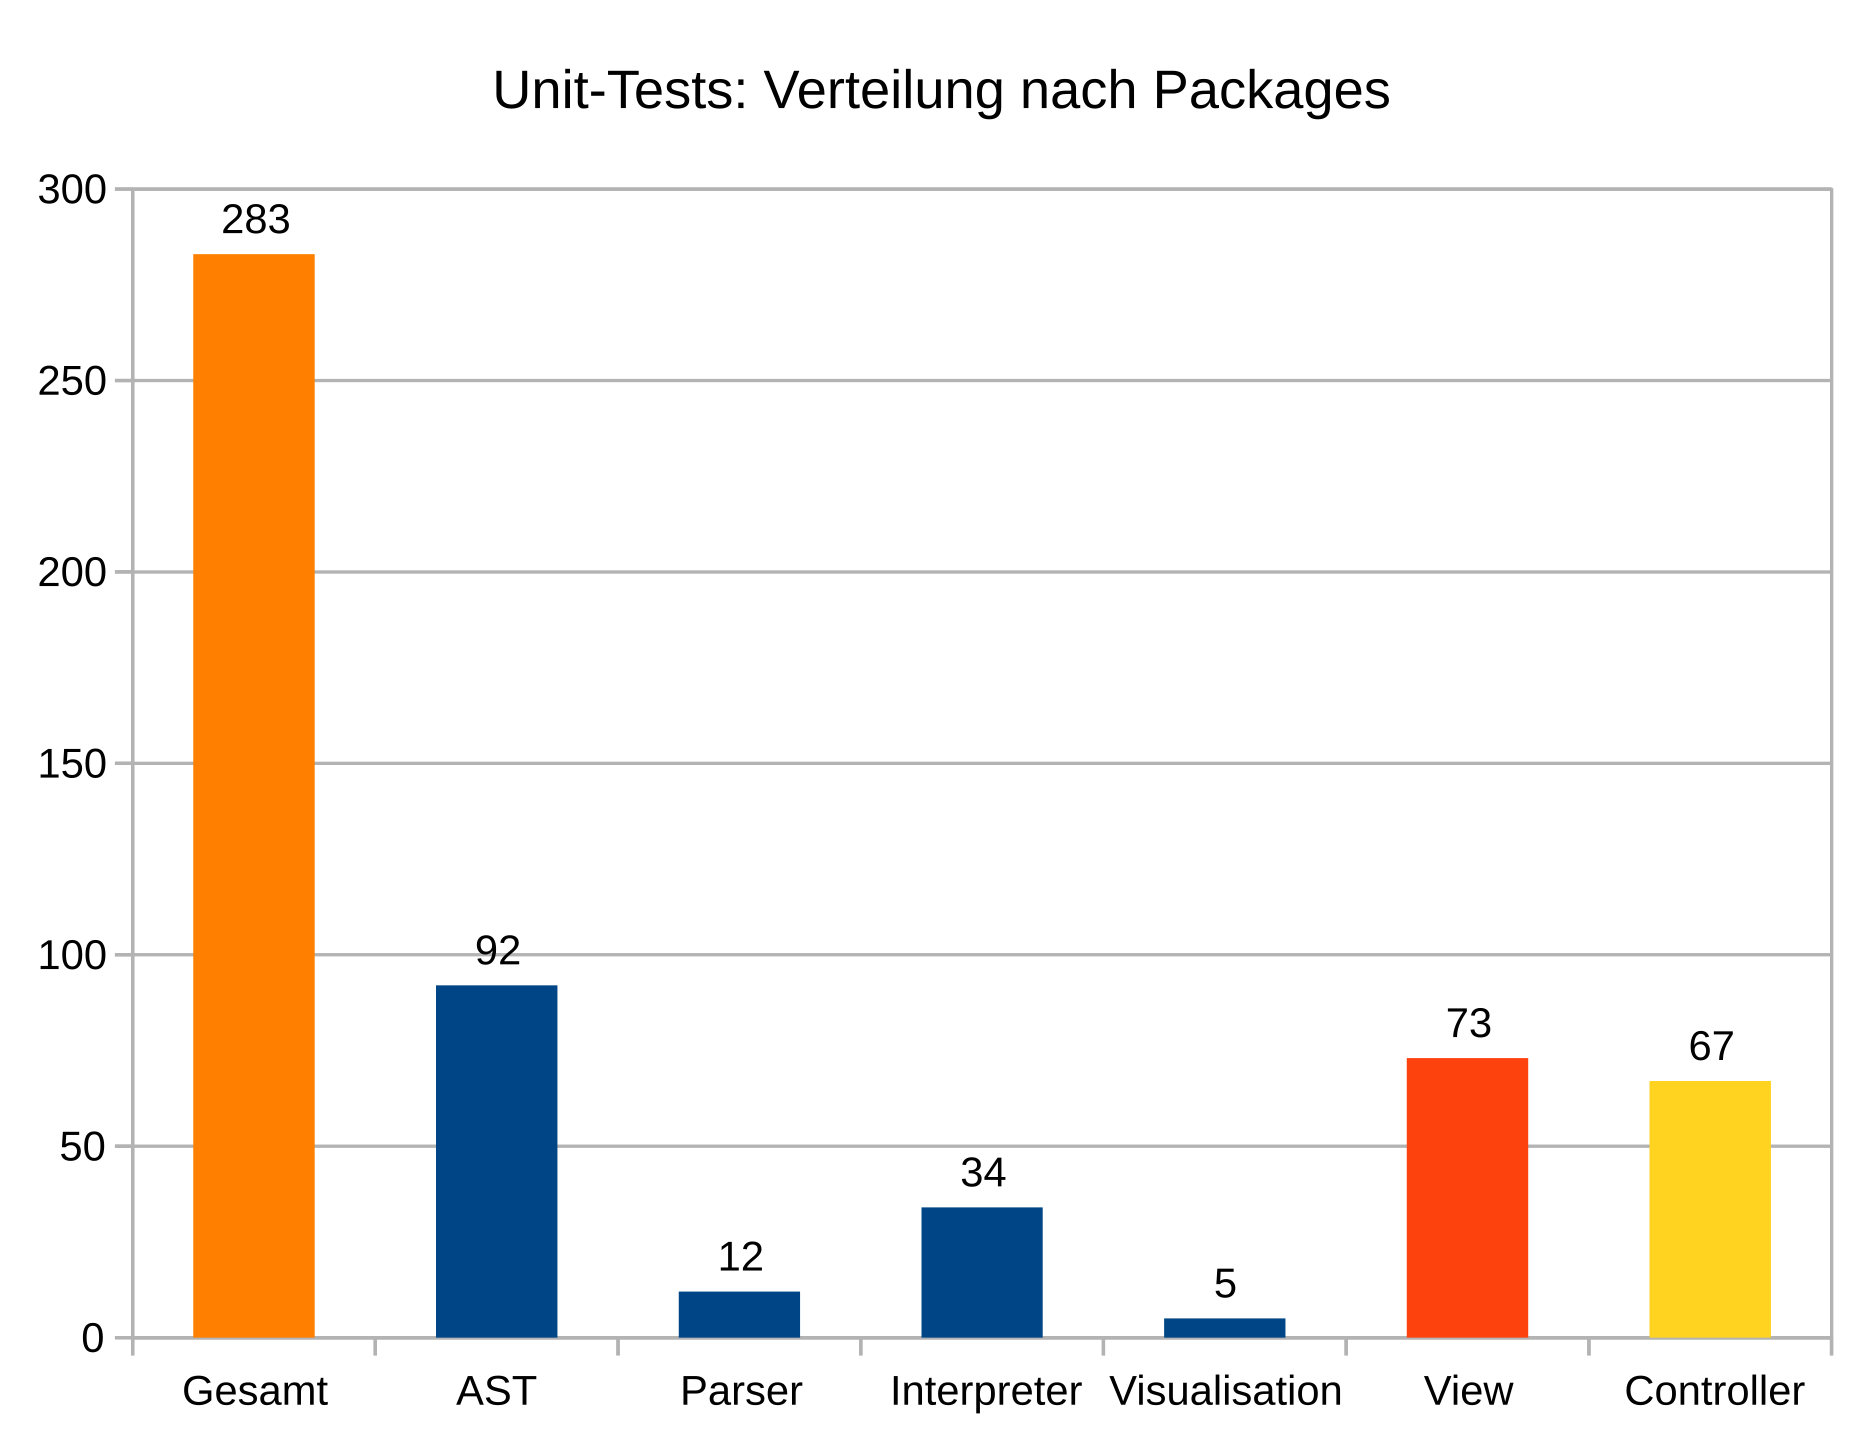
\includegraphics[width=0.75\linewidth]{images/tests_packages.png}
\end{figure}

\begin{figure}[!h]
	\centering
	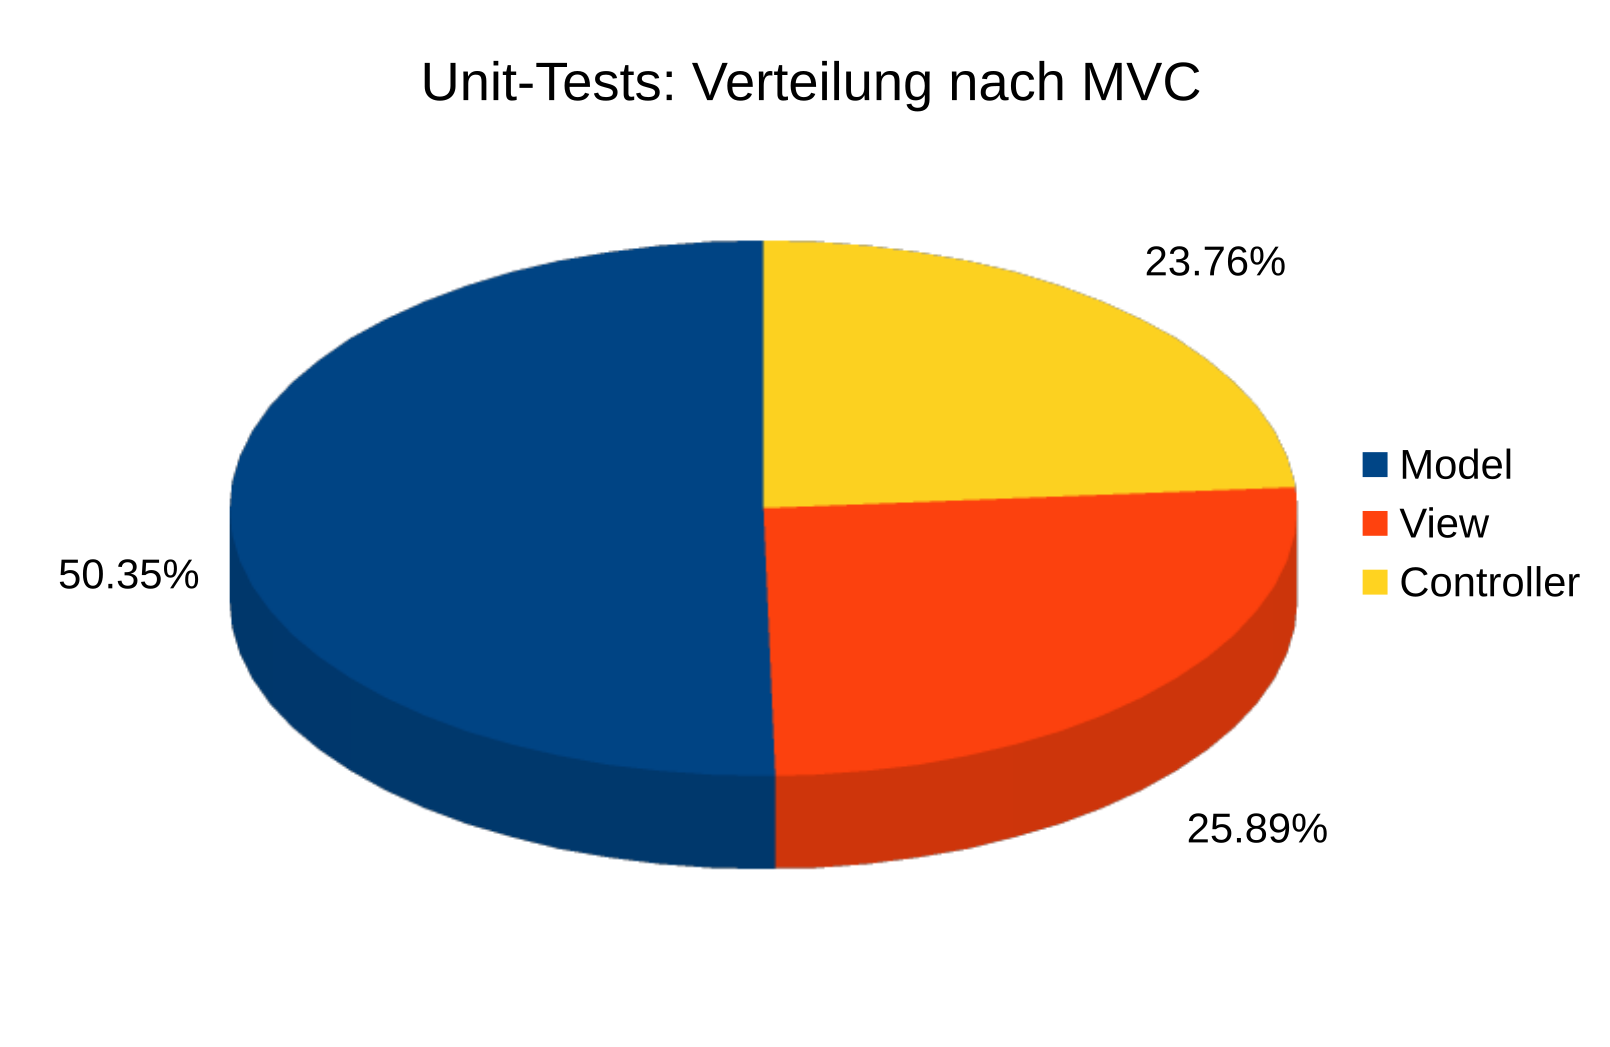
\includegraphics[width=0.7\linewidth]{images/tests_mvc.png}
\end{figure}

\subsection{Coverage}
Verteilung der Coverage auf einzelne Packages und die drei Komponenten des MVC-Architekturstils. Die Coverage berechnet auch die ignorierten Tests des Controllers mit ein, da diese prinzipiell funktionsfähig und nur durch einen Bug in einer Bibliothek eingeschränkt sind.

\begin{figure}[!h]
	\centering
	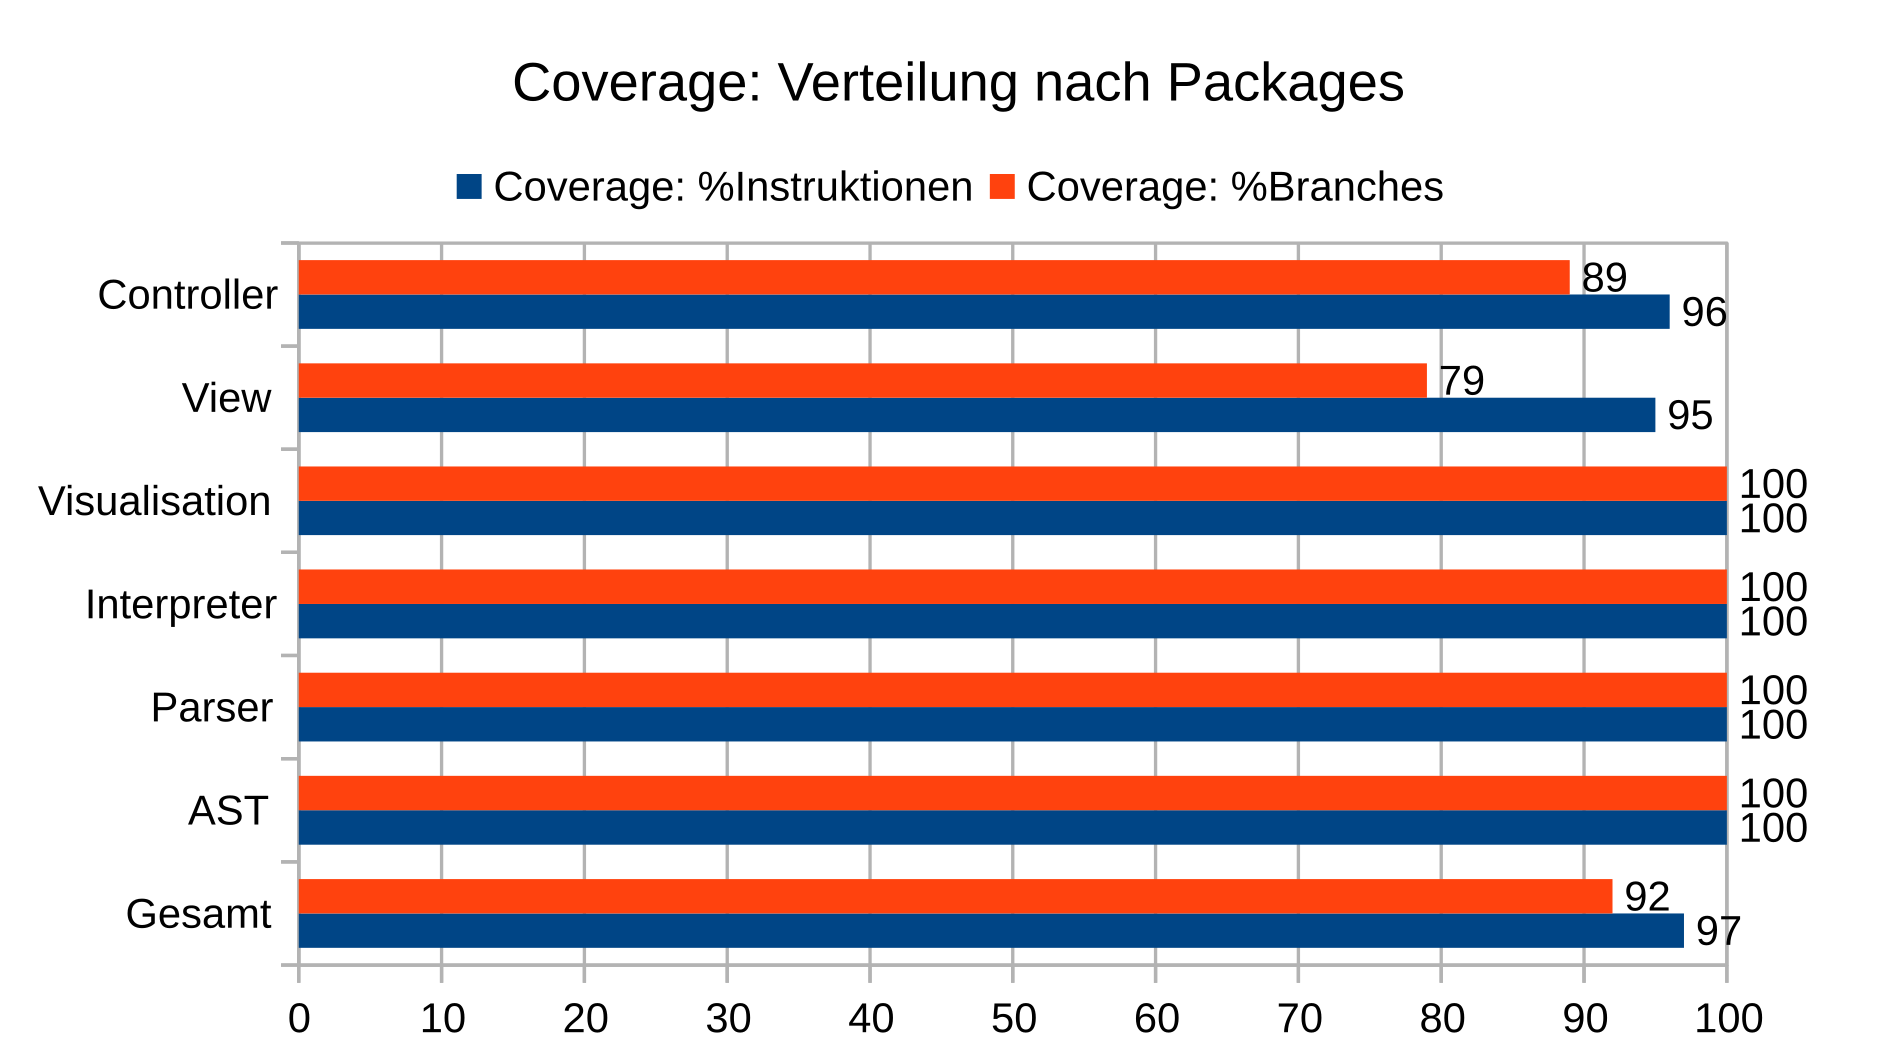
\includegraphics[width=\linewidth]{images/coverage_packages.png}
\end{figure}

\begin{figure}[!h]
	\centering
	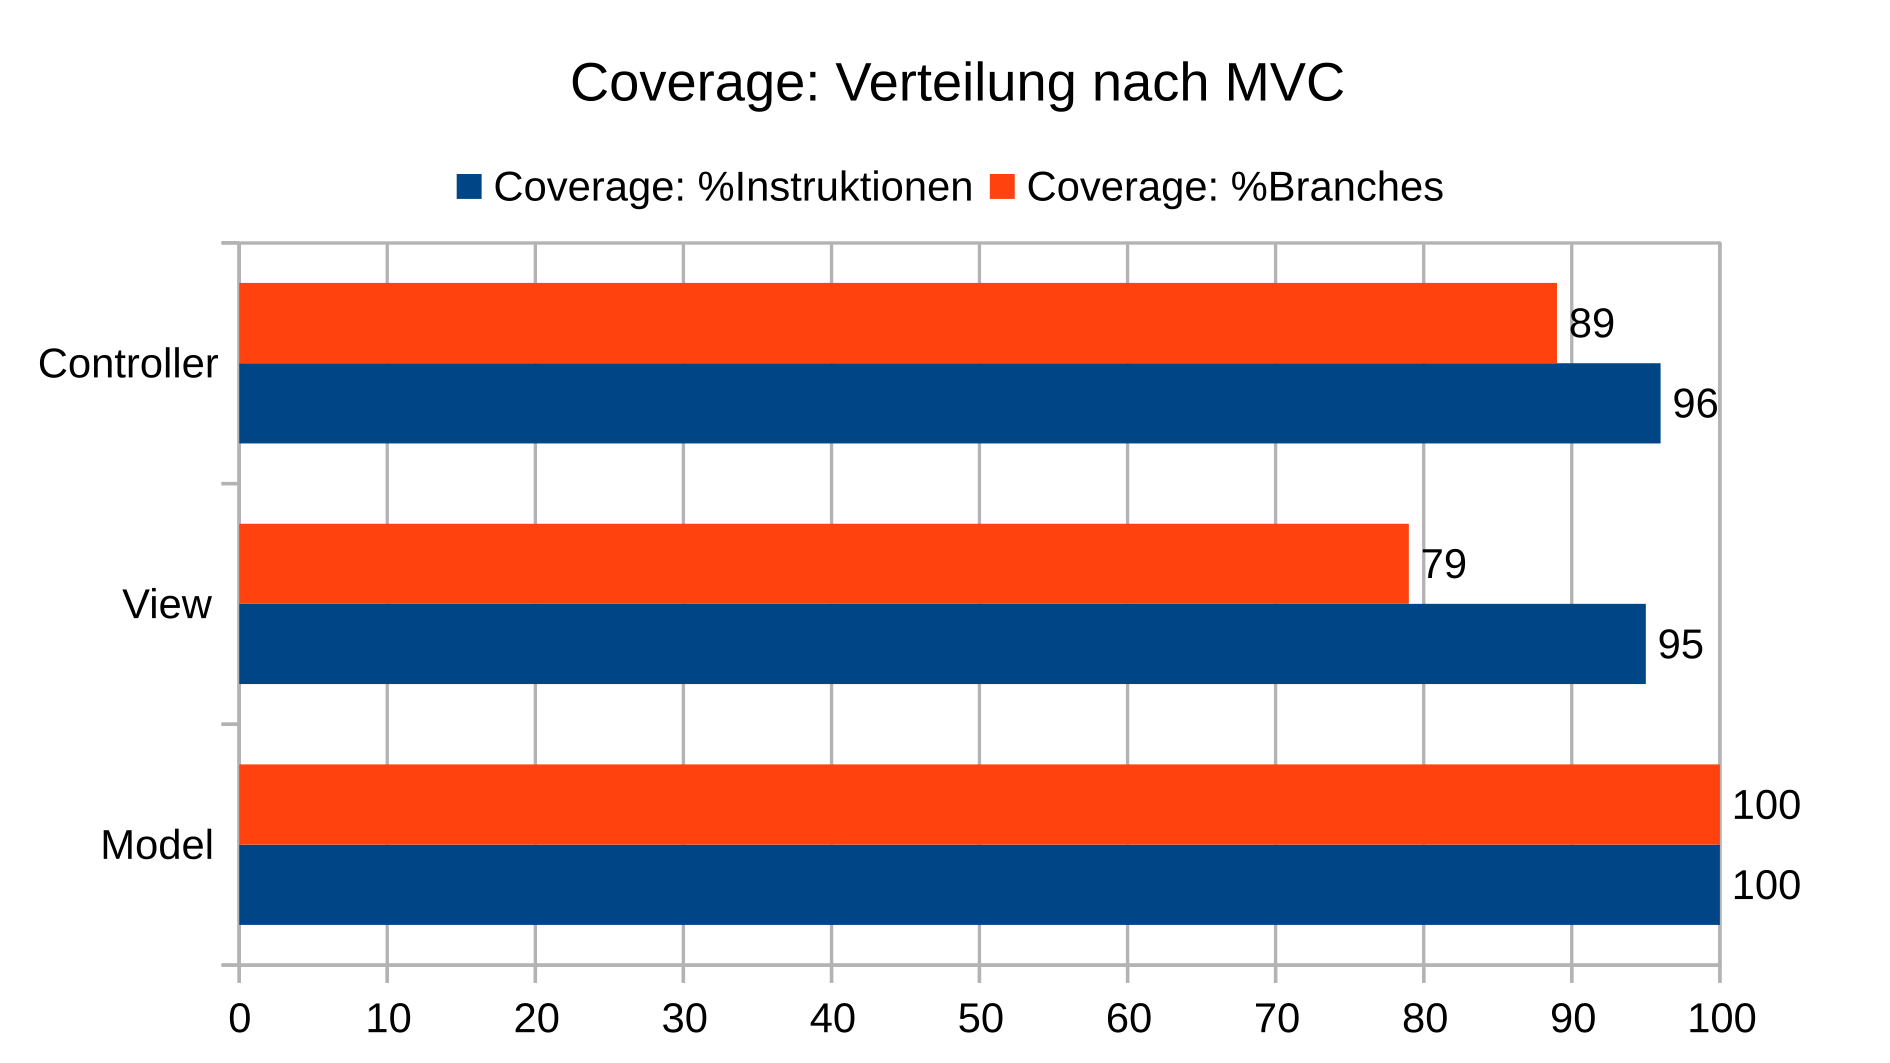
\includegraphics[width=\linewidth]{images/coverage_mvc.png}
\end{figure}

\subsection{Code-Verteilung in Hauptcode und Tests}
Verteilung des Codes auf die drei Komponenten des MVC-Architekturstils und das Model im Detail. Die Zeilenzahl berechnet auch die ignorierten Tests des Controllers mit ein, da diese prinzipiell funktionsfähig und nur durch einen Bug in einer Bibliothek eingeschränkt sind.

\begin{figure}[!h]
	\centering
	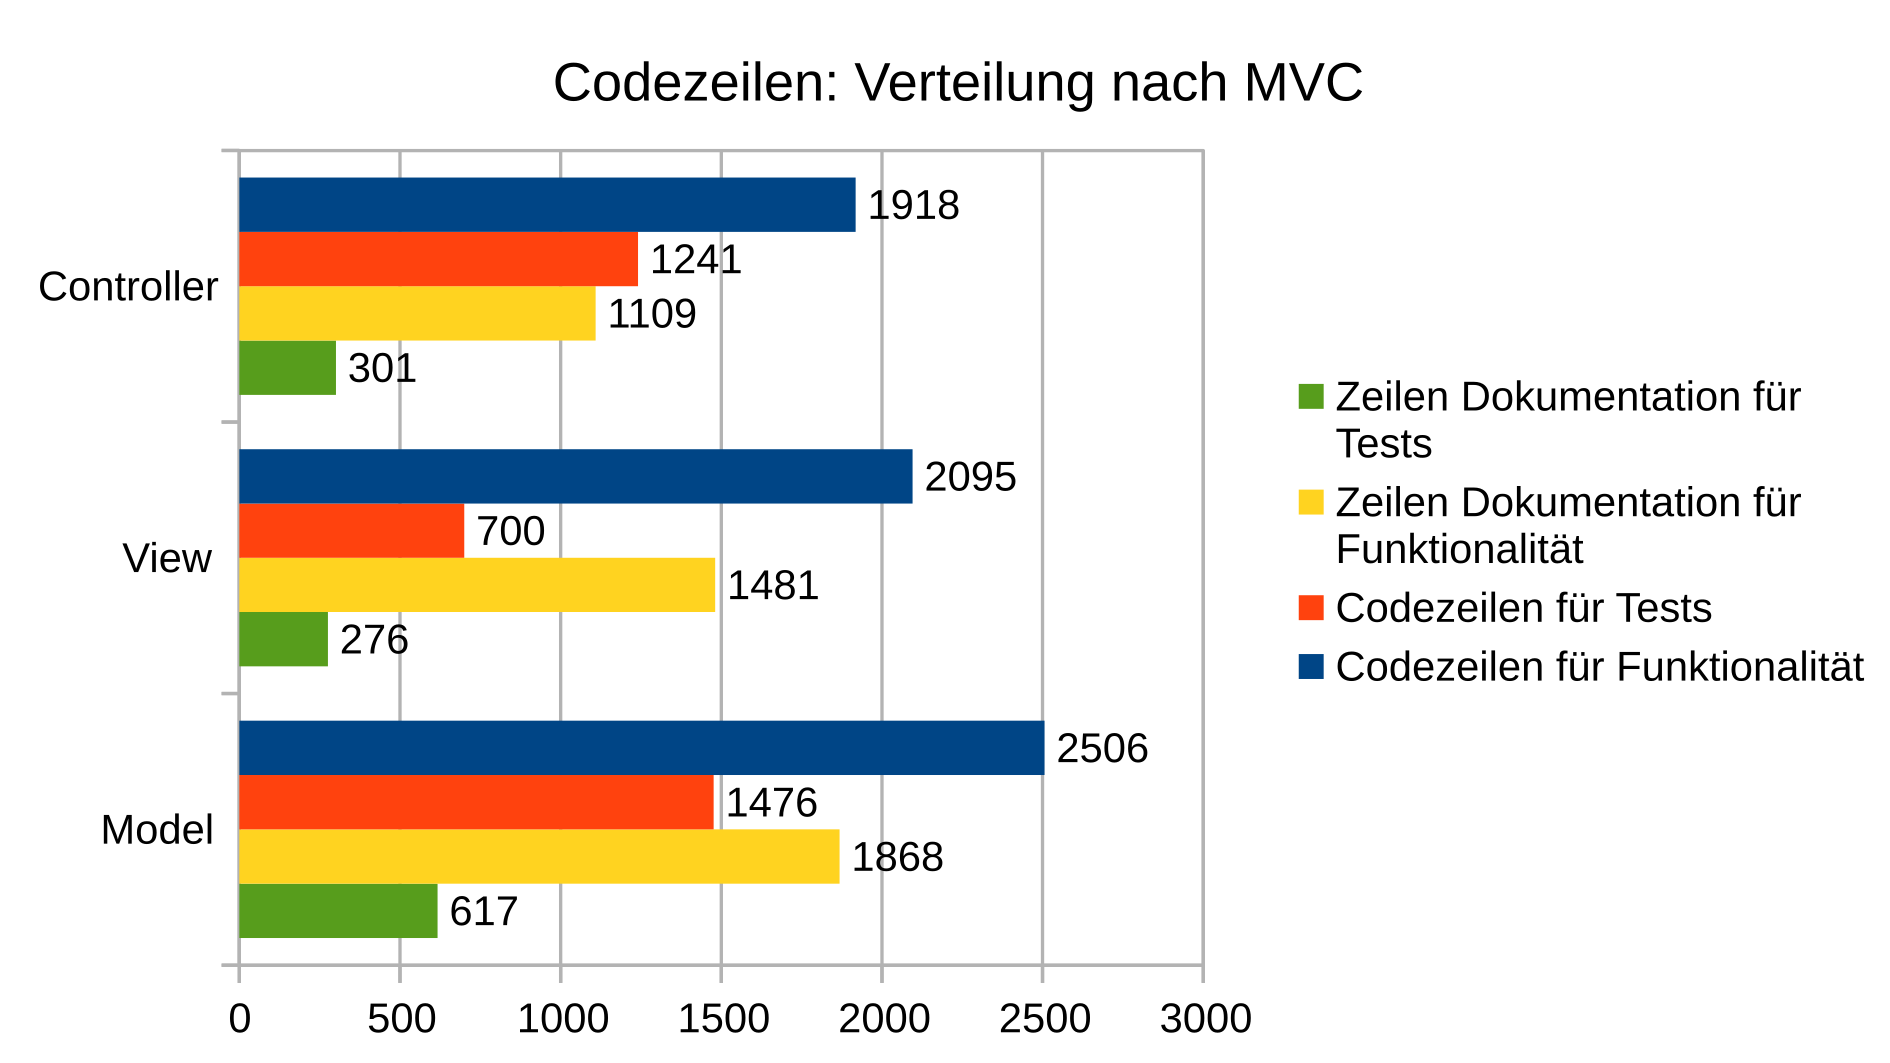
\includegraphics[width=\linewidth]{images/loc_mvc.png}
\end{figure}

\begin{figure}[!h]
	\centering
	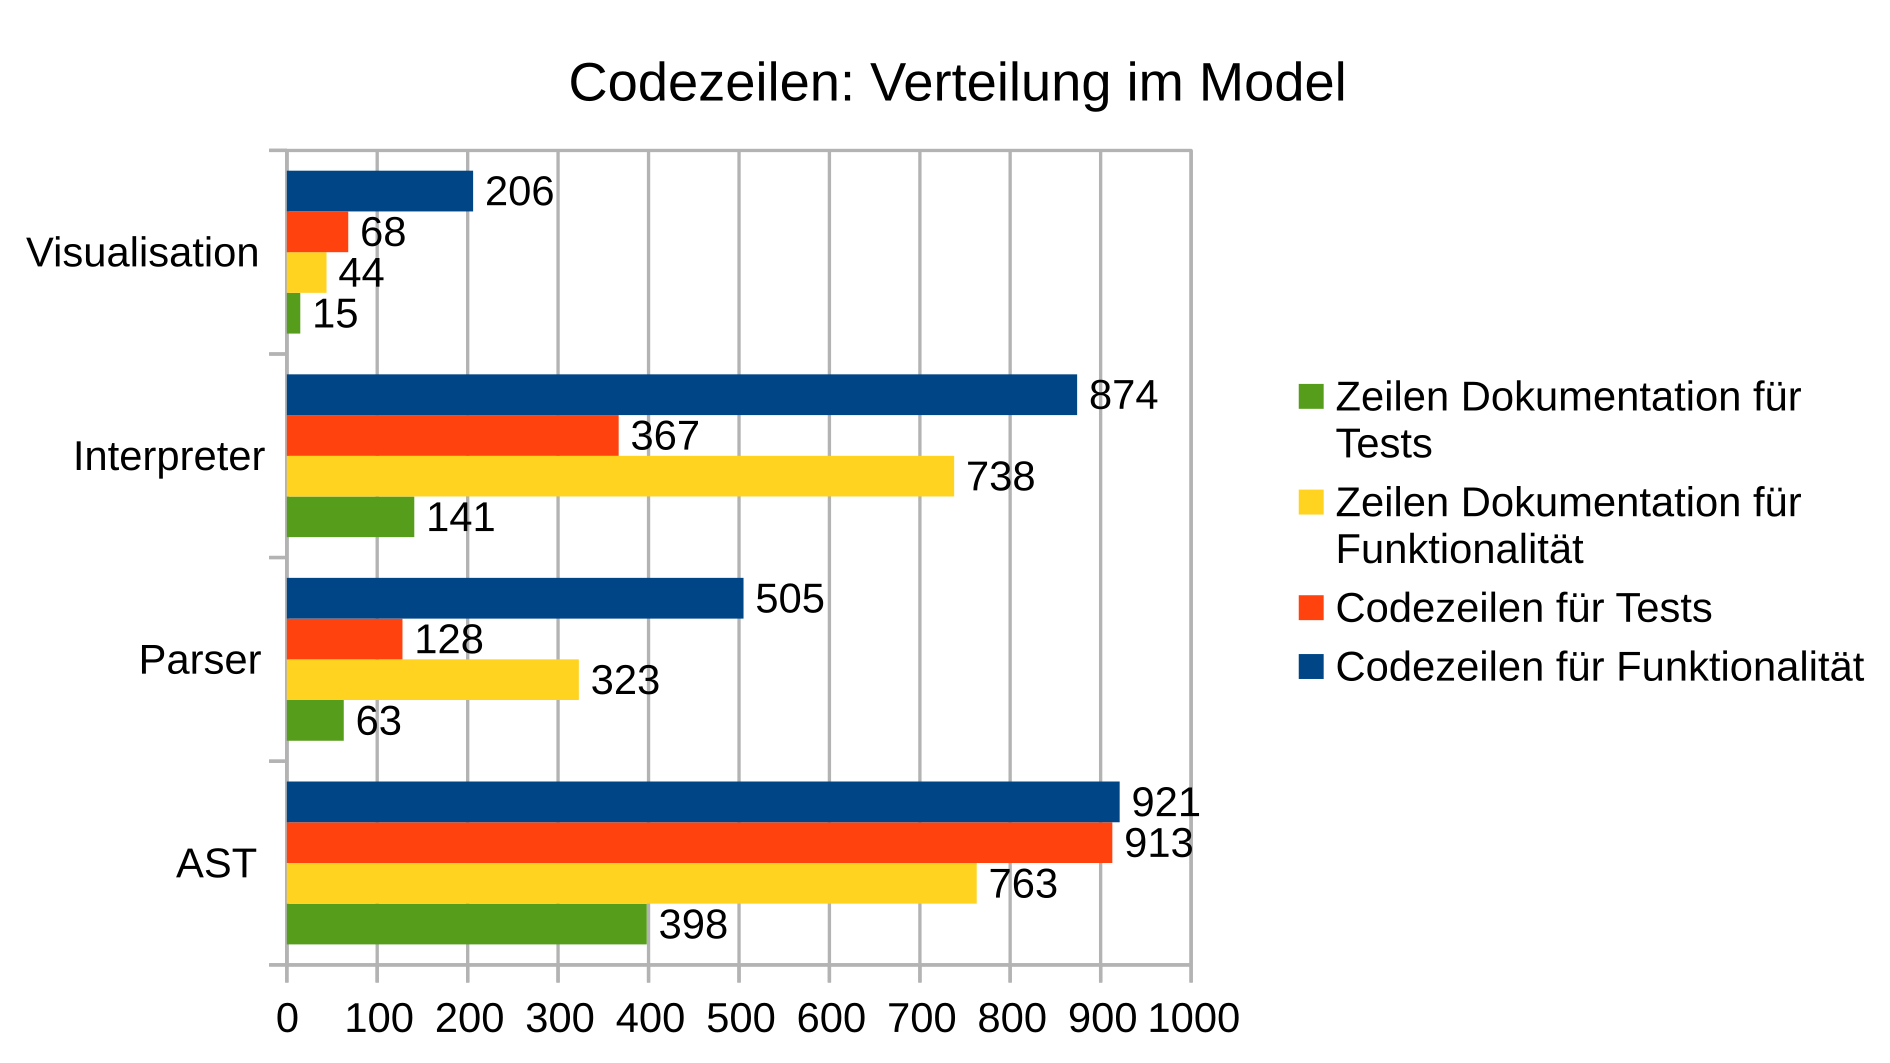
\includegraphics[width=\linewidth]{images/loc_model.png}
\end{figure}

\end{document}
